% !TEX encoding = UTF-8 Unicode
%用于展示
\documentclass[
10pt,
aspectratio=169,
]{beamer}
\newcommand{\Lorenz}{{\calligra Lorenz}}
\setbeamercovered{transparent=10}
\usetheme[
%  showheader,
%  red,
  purple,
%  gray,
%  graytitle,
  colorblocks,
%  noframetitlerule,
]{Verona}

\usepackage[T1]{fontenc}
\usepackage{tcolorbox}
\usepackage{circuitikz}
\usepackage[utf8]{inputenc}
\usepackage{cite} % 使用cite宏包来处理引用
\usepackage[numbers,authoryear]{natbib}  % 使用 natbib 包支持作者-年份引用
\usepackage{hyperref}  % 用于创建超链接
% \hypersetup{
%     colorlinks=true,        % 激活超链接的颜色
%     linkcolor=blue,         % 设置文献引用、目录等链接的颜色
%     urlcolor=blue,          % 设置URL的颜色
%     citecolor=blue          % 设置文献引用的颜色
% }
% 设置参考文献风格
\bibliographystyle{plain} % 指定样式
\usepackage{lipsum}
\definecolor{col}{RGB}{4,74,21}
%%%%%%%%%%%%%%%%%%%%%%%%%%%%%%%
% Mac上使用如下命令声明隶书字体,windows也有相关方式,大家可自行修改
\providecommand{\lishu}{\CJKfamily{zhli}}

% %%%%%%%%%%%%用于进行逐行显示%%%%%%%%%%%%%%%%%%%%%
% \setbeamertemplate{itemize items}[default] % 可选:更改列表符号样式
% \beamerdefaultoverlayspecification{<+->} % 默认逐项显示
% %%%%%%%%%%%%%%%%%%%%%%%%%%%%%%%%%%%%%%%%%%%%%%%%%%%
\usepackage{tikz}
\usetikzlibrary{fadings}
%
\setbeamertemplate{sections/subsections in toc}[ball]
\usepackage{xeCJK}
\usepackage{listings}
\usepackage{xcolor}

% 定义 Python 语言的样式
%\lstdefinestyle{mypython}适用于一个文章中有多个代码插入风格的情况
\lstset{
    language=Python,
    basicstyle=\small\ttfamily,  % 基本样式
    numbers=left,  % 左侧显示行号
    numberstyle=\footnotesize\itshape,  % 行号的样式
    stepnumber=1,
    numbersep=5pt,
    backgroundcolor=\color{gray!5}, % 代码块背景颜色
    showspaces=false,
    showstringspaces=false,
    showtabs=false,
    keywordstyle=\color{blue},
    commentstyle=\color{gray!50!black!50},    % 注释样式
    stringstyle=\rmfamily\slshape\color{red},  % 字符串样式
    frame=leftline, % 代码框形状
    rulecolor=\color{gray!90}, % 代码框颜色
    aboveskip=10pt,                % 框架上方的间距
    belowskip=10pt,                % 框架下方的间距
    framerule=12pt, 
    firstnumber=1,
    stepnumber=1,  % 若设置为2,则显示行号为1,3,5
    numbersep=7pt, % 行号与代码之间的间距
    aboveskip=.25em,  % 代码块边框
    showspaces=false,  % 显示添加特定下划线的空格
    keepspaces=true,
    showtabs=false,  % 在字符串中显示制表符
    % tabsize=2,  % 默认缩进2个字符
    %captionpos=b,  % 将标题位置设置为底部
    breaklines=true,  % 设置自动断行
    breakatwhitespace=false,  % 设置自动中断是否只发生在空格处
    breakautoindent=true,%不知道这句有什么用
    breakindent=1em,
    title=\lstname, 
    escapeinside=``,  % 在``里显示中文
    xleftmargin=1em, xrightmargin=1em, % 设定listing左右的空白
    aboveskip=1ex, belowskip=1ex,
    framextopmargin=1pt, framexbottommargin=1pt,
    abovecaptionskip=-2pt,belowcaptionskip=3pt,
    extendedchars=false, columns=flexible, mathescape=true,
    texcl=true,
    fontadjust
}
\usepackage{caption}
\usepackage{multicol}
\usepackage{calligra}
\setbeamertemplate{caption}[numbered]

\usepackage{subcaption}
\usefonttheme{professionalfonts}
\def\mathfamilydefault{\rmdefault}
\usepackage{amsmath}
\usepackage{multirow}
\usepackage{booktabs}
\usepackage{bm}
\setbeamertemplate{section in toc}{\hspace*{1em}\inserttocsectionnumber.~\inserttocsection\par}
\setbeamertemplate{subsection in toc}{\hspace*{2em}\inserttocsectionnumber.\inserttocsubsectionnumber.~\inserttocsubsection\par}
\setbeamerfont{subsection in toc}{size=\small}
\AtBeginSection[]{%
	\begin{frame}%
		\frametitle{目录}%
        \begin{multicols}{2}
            \textbf{\tableofcontents[currentsection]} %
            \end{multicols}
		
	\end{frame}%
}

\AtBeginSubsection[]{%
	\begin{frame}%
		\frametitle{目录}%
        \begin{multicols}{2}
            \textbf{\tableofcontents[currentsection, currentsubsection]} %
        \end{multicols}
\end{frame}%
}

\title{基于多智能体协作的异构配送仿真系统}
\subtitle{无人机、无人车、机器狗协同配送建模与实现}
\author[崔迪生,黄皓凌,岑岱,李梓琳,李家龙]
{崔迪生,黄皓凌,岑岱,李梓琳,李家龙}
\mail{cuidsh@mail2.sysu.edu.cn}
\institute[中山大学]{中山大学\\
系统科学与工程学院\\
指导老师:李雄
}
\date{2024.6.18}

\titlegraphic[width=3cm]{sysu_logo}{}



%%%%%%%%%%%%%%%%%%%%%%%%%%%%%%%%
% ----------- 标题页 ------------
%%%%%%%%%%%%%%%%%%%%%%%%%%%%%%%%


% 这部分是定制页面的标题栏(headlines),用于显示章节信息
\setbeamertemplate{headline}{
    \begin{beamercolorbox}[ht=2.5ex, left, wd=\paperwidth, sep=0pt, colsep=1ex]{section in head/foot}
        \usebeamerfont{section in head/foot}
        \insertsectionhead/
        \insertsubsectionhead/
        \insertsubsubsectionhead
      \end{beamercolorbox}
    
}

\begin{document}
\maketitle

\begin{frame}
    {目录}
    \begin{multicols}{2}
        \tableofcontents
        \end{multicols}
\end{frame}
%%%%%%%%%%%%%%%%%%%%%%%%%%%%%%%%
% ----------- Temp ------------
%%%%%%%%%%%%%%%%%%%%%%%%%%%%%%%%

% \begin{exampleblock}{title}
% 		xxx
% 	\end{exampleblock}

% \begin{columns}[onlytextwidth]
% 		\begin{column}{.5\textwidth}
% 		\end{column}
% \end{columns}

% \begin{figure}
% 		\centering
% 		\includegraphics[width=0.8\linewidth]{fig/intro_private.png}
% 		\caption{Privacy security policy}
% \end{figure}

% \begin{equation*}
% 		w=\sum _{j=1}^{M}\frac{\left | \mathcal{D}_j \right | w_j^e}{\sum _{j=1}^{M}\left | \mathcal{D}_j \right |}
% \end{equation*}

%%%%%%%%%%%%%%%%%%%%%%%%%%%%%%%%
% ----------- FRAME ------------
%%%%%%%%%%%%%%%%%%%%%%%%%%%%%%%%

%-----------cend-----------S
\section{系统概述}

\subsection{研究背景与动机}

\begin{frame}{研究背景与动机}
    \begin{columns}
        \begin{column}{0.25\textwidth}
            \begin{figure}
                \centering
                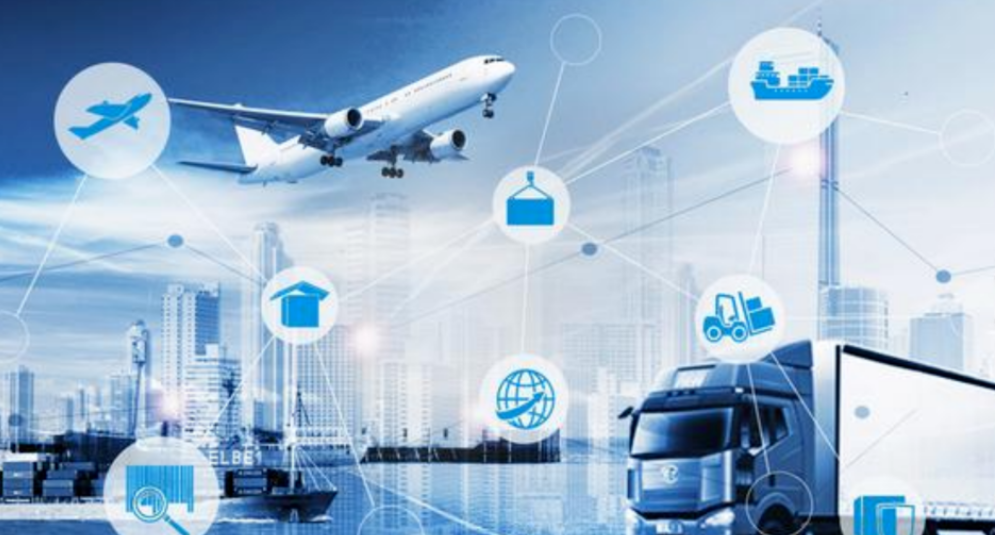
\includegraphics[width=\linewidth]{background.png}
                \caption{配送系统场景}
            \end{figure}
        \end{column}
        \begin{column}{0.25\textwidth}
            \begin{block}{现实挑战}
                \begin{itemize}
                    \item 城市交通拥堵严重
                    \item 配送需求指数增长
                    \item 复杂地形配送困难
                    \item 单一载具效率有限
                \end{itemize}
            \end{block}
        \end{column}
        \begin{column}{0.25\textwidth}
            \begin{alertblock}{技术机遇}
                \begin{itemize}
                    \item 多智能体技术成熟
                    \item 异构协作潜力巨大
                    \item 分布式决策鲁棒
                    \item 智能算法优化效率
                \end{itemize}
            \end{alertblock}
        \end{column}
        \begin{column}{0.25\textwidth}
            \begin{exampleblock}{研究目标}
                \textbf{核心目标:}构建异构智能体协作的城市配送仿真系统
                
                \textbf{技术价值:}
                \begin{itemize}
                    \item 提高配送效率
                    \item 降低运营成本
                    \item 增强容错能力
                    \item 支持应急救援
                \end{itemize}
            \end{exampleblock}
        \end{column}
    \end{columns}
\end{frame}

\subsection{相关技术综述}

\begin{frame}{多智能体系统技术基础}
    \begin{block}{核心技术领域}
        \begin{description}
            \item[多智能体协作] 分布式决策、任务分配、协商机制
            \item[路径规划算法] A*算法、动态路径重规划、启发式搜索
            \item[异构系统融合] 不同能力智能体的优势互补与协同
            \item[实时仿真技术] 高频更新、可视化渲染、性能监控
        \end{description}
    \end{block}
    
    \begin{alertblock}{技术创新点}
        \begin{itemize}
            \item \textbf{双策略决策机制}:直达与中转策略智能选择
            \item \textbf{战争迷雾探索}:有限视野下的协作式地图构建
            \item \textbf{紧急度权重算法}:基于任务优先级的动态调度
            \item \textbf{异构载具建模}:真实物理特性的精确仿真
        \end{itemize}
    \end{alertblock}
\end{frame}

%%%%%%%%%%%%%%%%%%%%%%%%%%%%%%%%
% ----------- 建模思路 ----------
%%%%%%%%%%%%%%%%%%%%%%%%%%%%%%%%
\section{基于BDI的建模}

\section{建模思路}

\subsection{异构智能体设计}

\begin{frame}{三种智能体类型}
    \begin{block}{智能体能力对比}
        \begin{center}
        \begin{tabular}{|c|c|c|c|c|}
        \hline
        \textbf{智能体} & \textbf{速度} & \textbf{载重} & \textbf{地形适应} & \textbf{特殊能力} \\
        \hline
        无人机(Drone) & 15.0 & 10kg & 全地形 & 飞行、跨水域 \\
        \hline
        无人车(Car) & 5.0 & 50kg & 仅道路 & 大载重运输 \\
        \hline
        机器狗(RobotDog) & 7.0 & 30kg & 陆地全地形 & 爬坡、攀爬 \\
        \hline
        \end{tabular}
        \end{center}
    \end{block}
    
    \begin{columns}
        \begin{column}{0.5\textwidth}
            \begin{exampleblock}{核心能力}
                \begin{itemize}
                    \item 自主路径跟踪与移动
                    \item 有限视野环境探索(半径=5)
                    \item 状态管理:idle→delivering→returning
                    \item 实时位置与任务状态上报
                \end{itemize}
            \end{exampleblock}
        \end{column}
        \begin{column}{0.5\textwidth}
            \begin{exampleblock}{协作机制}
                \begin{itemize}
                    \item 共享环境知识发现
                    \item 动态任务分配与重分配
                    \item 中转站协作配送
                    \item 智能返回路径选择
                \end{itemize}
            \end{exampleblock}
        \end{column}
    \end{columns}
\end{frame}

\subsection{双策略决策机制}

\begin{frame}{智能决策策略总览}
    \begin{block}{双策略决策机制:        系统为每个任务计算两种策略的成本}

        \begin{enumerate}
            \item \textbf{直达策略}: 智能体直接从仓库配送到目标
            \item \textbf{中转策略}: 通过中转站进行两段式配送
        \end{enumerate}
    \end{block}
    
    \begin{columns}
        \begin{column}{0.5\textwidth}
            \begin{alertblock}{决策算法核心}
                \begin{equation}
                \text{Strategy} = \begin{cases}
                \text{Direct} & \text{if } C_{direct} \leq C_{relay} \\
                \text{Relay} & \text{if } C_{direct} > C_{relay}
                \end{cases}
                \end{equation}
                
                其中:$C = \frac{\text{路径成本}}{\text{紧急度权重}}$
            \end{alertblock}
        \end{column}
        \begin{column}{0.5\textwidth}
            \begin{exampleblock}{紧急度权重公式}
                \begin{align}
                    w_{urgency} &= 1 + u \\
                    C_{total} &= \frac{C_{path}}{w_{urgency}}
                \end{align}
                \begin{itemize}
                    \item $u$: 任务紧急度 (1-5级)
                    \item $C_{path}$: 原始路径成本
                    \item $C_{total}$: 最终调整后成本
                \end{itemize}
            \end{exampleblock}
        \end{column}
    \end{columns}
\end{frame}

\begin{frame}{双策略决策机制数学模型}
    \begin{columns}
        \begin{column}{0.5\textwidth}
            \begin{block}{直达策略成本公式}
                \begin{align}
                    C_{direct} &= \frac{C_{a \to w} + C_{w \to g}}{1 + u} \\
                    \text{where:} \\
                    C_{a \to w} &= \frac{d(a,w)}{v_a} \\
                    C_{w \to g} &= \frac{d(w,g)}{v_a}
                \end{align}
                
                \begin{itemize}
                    \item $a$: 智能体当前位置
                    \item $w$: 仓库位置
                    \item $g$: 目标位置
                    \item $v_a$: 智能体速度
                    \item $u$: 任务紧急度
                \end{itemize}
            \end{block}
        \end{column}
        \begin{column}{0.5\textwidth}
            \begin{alertblock}{中转策略成本公式}
                \begin{align}
                    C_{relay} &= \frac{C_{leg1} + C_{leg2} + P_{wait}}{1 + u} \\
                    \text{where:} \\
                    C_{leg1} &= \frac{d(a,w) + d(w,r)}{v_{a1}} \\
                    C_{leg2} &= \frac{d(r,g)}{v_{a2}}
                \end{align}
                
                \begin{itemize}
                    \item $r$: 中转站位置
                    \item $v_{a1},v_{a2}$: 第一、二阶段智能体速度
                    \item $P_{wait}$: 等待惩罚系数
                \end{itemize}
            \end{alertblock}
        \end{column}
    \end{columns}
    
    \begin{exampleblock}{优先级队列调度公式}
        任务队列中的任务按优先级 $p$ 排序:$p = -u + \frac{t_{\text{arrival}}}{10000}$,紧急度越高优先级值越小,越优先
    \end{exampleblock}
\end{frame}

\subsection{路径规划算法}
\begin{frame}{A*算法基本原理}
    \begin{alertblock}{核心评估函数}
        \begin{align}
            f(n) &= g(n) + h(n) \\
            g(n) &= \text{起点到节点}n\text{的实际成本} \\
            h(n) &= \text{节点}n\text{到目标的估计成本}
        \end{align}
    \end{alertblock}
    
    \begin{columns}
        \begin{column}{0.5\textwidth}
            \begin{exampleblock}{启发式函数}
                \begin{equation}
                    h(n) = \sqrt{(n_x - g_x)^2 + (n_y - g_y)^2}
                \end{equation}
                
                满足可接受性条件:$h(n) \leq h^*(n)$
            \end{exampleblock}
        \end{column}
        \begin{column}{0.5\textwidth}
            \begin{alertblock}{算法特性}
                \begin{itemize}
                    \item 最优性保证
                    \item 8方向搜索
                    \item 动态障碍处理
                    \item 多智能体适配
                \end{itemize}
            \end{alertblock}
        \end{column}
    \end{columns}
\end{frame}

\begin{frame}{地形成本模型}
    \begin{block}{路径成本计算}
        \begin{equation}
            g_{new}(n) = g(m) + w_{move} + P_{terrain} + P_{unknown}
        \end{equation}
    \end{block}
    
    \begin{columns}
        \begin{column}{0.5\textwidth}
            \begin{exampleblock}{地形惩罚系数}
                \begin{align}
                    P_{terrain} = \begin{cases}
                    0 & \text{道路} \\
                    2 & \text{山地} \\
                    5 & \text{陡峭地形} \\
                    \infty & \text{禁止区域}
                    \end{cases}
                \end{align}
            \end{exampleblock}
        \end{column}
        \begin{column}{0.5\textwidth}
            \begin{alertblock}{未知区域处理}
                \begin{equation}
                    P_{unknown} = 10 \times \mathbb{I}_{unknown}(n)
                \end{equation}
                其中 $\mathbb{I}_{unknown}(n)$ 为未知区域指示函数
            \end{alertblock}
        \end{column}
    \end{columns}
    
    \begin{exampleblock}{路径终止条件}
        \begin{equation}
            \|pos_{end} - pos_{goal}\| \leq \epsilon, \quad \epsilon = 5.0
        \end{equation}
    \end{exampleblock}
\end{frame}

\begin{frame}{智能体约束适配}
    \begin{block}{差异化通行能力}
        \begin{equation}
            accessible(agent, terrain) = \begin{cases}
            \text{True} & \text{if } agent \in \{drone\} \\
            terrain \neq water & \text{if } agent \in \{car, robot\_dog\}
            \end{cases}
        \end{equation}
    \end{block}
    
    \begin{columns}
        \begin{column}{0.5\textwidth}
            \begin{exampleblock}{移动成本权重}
                \begin{align}
                    w_{move} &= \begin{cases}
                    1.0 & \text{直线移动} \\
                    \sqrt{2} & \text{对角移动}
                    \end{cases}
                \end{align}
            \end{exampleblock}
        \end{column}
        \begin{column}{0.5\textwidth}
            \begin{alertblock}{性能优化}
                \begin{itemize}
                    \item 优先队列管理:$O(\log n)$
                    \item 邻居遍历:8方向搜索
                    \item 路径重构:父节点回溯
                    \item 内存优化:访问标记
                \end{itemize}
            \end{alertblock}
        \end{column}
    \end{columns}
\end{frame}

\subsection{多智能体协调}

\begin{frame}{多智能体协调算法}
    \begin{block}{协调系统核心功能}
        \begin{itemize}
            \item \textbf{任务队列管理}: 基于优先队列的紧急度排序
            \item \textbf{智能体状态监控}: 实时追踪所有智能体状态
            \item \textbf{路径规划服务}: 为智能体提供最优路径计算
            \item \textbf{中转站协调}: 管理两阶段协作配送流程
        \end{itemize}
    \end{block}
    
    \begin{columns}
        \begin{column}{0.5\textwidth}
            \begin{alertblock}{系统更新频率}
                \begin{equation}
                f_{update} = 50 Hz \Rightarrow T_{frame} = 20 ms
                \end{equation}
            \end{alertblock}
        \end{column}
        \begin{column}{0.5\textwidth}
            \begin{exampleblock}{任务调度模型}
                \begin{align}
                p_i &= -u_i + \frac{t_{arrival}^i}{10000} \\
                task^* &= \arg\min_{task_i \in Q} p_i
                \end{align}
            \end{exampleblock}
        \end{column}
    \end{columns}
\end{frame}

\begin{frame}{多智能体协调算法公式}
    \begin{columns}
        \begin{column}{0.5\textwidth}
            \begin{exampleblock}{任务优先级队列}
                任务优先级计算:
                \begin{align}
                P(task) &= U_{base} \cdot w_{urgency} + w_{time} \cdot T_{wait} \\
                U_{base} &= 5 \cdot \text{task.urgency} \\
                T_{wait} &= t_{current} - t_{arrival}
                \end{align}
                其中$w_{urgency}$和$w_{time}$为权重系数
            \end{exampleblock}
        \end{column}
        \begin{column}{0.5\textwidth}
            \begin{alertblock}{智能体分配效用函数}
                \begin{align}
                U(agent, task) &= \frac{C_{capability} \cdot C_{availability}}{C_{distance}} \\
                C_{capability} &= 
                \begin{cases}
                1.0, & \text{if } w_{task} \leq w_{agent.max} \\
                0.0, & \text{otherwise}
                \end{cases} \\
                C_{availability} &= 1 - \frac{t_{busy}}{t_{total}}
                \end{align}
            \end{alertblock}
        \end{column}
    \end{columns}
\end{frame}

\begin{frame}{协调系统最优分配算法}
    \begin{block}{协调系统状态转移}
        智能体状态转移概率矩阵:
        \begin{align}
        P = \begin{pmatrix}
        0.7 & 0.2 & 0.1 \\
        0.1 & 0.8 & 0.1 \\
        0.2 & 0.1 & 0.7
        \end{pmatrix}
        \end{align}
        状态空间:\{idle, delivering, returning\}
    \end{block}
    
    \begin{alertblock}{最优协调分配}
        \begin{align}
        A^* = \underset{A}{\arg\max} \sum_{i=1}^{n} \sum_{j=1}^{m} U(agent_i, task_j) \cdot a_{ij}
        \end{align}
        约束:$\sum_{j=1}^{m} a_{ij} \leq 1, \forall i \in \{1,2,...,n\}$,$a_{ij} \in \{0,1\}$
    \end{alertblock}
\end{frame}

\subsection{环境建模}

\begin{frame}{地图系统设计}
    \begin{block}{Map类功能}
        \begin{itemize}
            \item \textbf{程序化地形生成}: 使用Perlin噪声创建真实地形
            \item \textbf{多层次地形}: 道路、水域、山地、建筑、植被6种类型
            \item \textbf{动态天气系统}: 晴天、雨天、雪天影响智能体性能
            \item \textbf{战争迷雾机制}: 智能体有限视野逐步探索
        \end{itemize}
    \end{block}
    
    \begin{columns}
        \begin{column}{0.5\textwidth}
            \begin{exampleblock}{SharedKnowledgeMap}
                \begin{itemize}
                    \item 共享环境知识库
                    \item 批量信息更新
                \end{itemize}
            \end{exampleblock}
        \end{column}
        \begin{column}{0.5\textwidth}
            \begin{alertblock}{探索机制}
                \begin{itemize}
                    \item 探索半径:5单位
                    \item 渐进式地图构建
                \end{itemize}
            \end{alertblock}
        \end{column}
    \end{columns}
\end{frame}

\begin{frame}{环境模型与战争迷雾}
    \begin{columns}
        \begin{column}{0.5\textwidth}
            \begin{exampleblock}{战争迷雾模型}
                智能体可视区域:
                \begin{align}
                V(agent) &= \{(x,y) | d(p_{agent}) \leq r_{vision}\} \\
                K_t(x,y) &= 
                \begin{cases}
                Terrain(x,y), & \text{if explored} \\
                K_{t-1}(x,y), & \text{otherwise}
                \end{cases}
                \end{align}
            \end{exampleblock}
        \end{column}
        \begin{column}{0.5\textwidth}
            \begin{alertblock}{Perlin地形生成}
                \begin{align}
                P(x,y) &= \sum_{i=1}^{n} w_i \cdot p_i(x \cdot 2^i, y \cdot 2^i) \\
                \text{Terrain}(x,y) &= 
                \begin{cases}
                \text{水域}, & P < -0.4 \\
                \text{平地}, & -0.4 \leq P < 0.1 \\
                \text{山地}, & P \geq 0.1
                \end{cases}
                \end{align}
            \end{alertblock}
        \end{column}
    \end{columns}
\end{frame}

\subsection{可视化与日志}
\begin{frame}{实时可视化系统}
    \begin{block}{DeliveryVisualizer核心功能}
        \begin{itemize}
            \item \textbf{高性能动画}: Matplotlib动画,blit=True优化
            \item \textbf{交互控制}: 支持暂停、继续、速度调整
            \item \textbf{实时监控}: 50FPS刷新率,状态实时显示
        \end{itemize}
    \end{block}
    
    \begin{columns}
        \begin{column}{0.5\textwidth}
            \begin{exampleblock}{可视化更新公式}
                \begin{align}
                    I_{map}(t) &= \mathcal{V}(K_t) \\
                    \forall a_i \in A: P_i(t) &= \mathcal{M}(a_i.pos, t)
                \end{align}
                其中:
                \begin{itemize}
                    \item $I_{map}(t)$: 地图可视化状态
                    \item $P_i(t)$: 智能体位置渲染
                    \item 更新频率: 50FPS
                \end{itemize}
            \end{exampleblock}
        \end{column}
        \begin{column}{0.5\textwidth}
            \begin{alertblock}{日志分析统计}
                任务性能统计公式:
                \begin{align}
                \bar{T} &= \frac{1}{n}\sum_{i=1}^{n}(T_{end}^i - T_{start}^i) \\
                \sigma_T &= \sqrt{\frac{1}{n}\sum_{i=1}^{n}(T_i - \bar{T})^2}
                \end{align}
                
                支持实时性能监控和任务完成统计分析
            \end{alertblock}
        \end{column}
    \end{columns}
\end{frame}

\begin{frame}{性能评估指标与数据分析公式}
    \begin{columns}
        \begin{column}{0.5\textwidth}
            \begin{exampleblock}{配送效率指标}
                任务完成时间效率:
                \begin{align}
                E_{time} &= \frac{1}{N} \sum_{i=1}^{N} \frac{T_{expected}(i)}{T_{actual}(i)} \\
                T_{expected}(i) &= \frac{d(s_i, g_i)}{v_{agent}} \cdot \alpha_{terrain}
                \end{align}
                
                策略选择正确率:
                \begin{align}
                ACC_{strategy} &= \frac{|\{i | C_{i,selected} \leq C_{i,alternative}\}|}{N} \\
                \end{align}
            \end{exampleblock}
        \end{column}
        \begin{column}{0.5\textwidth}
            \begin{alertblock}{负载均衡评估}
                智能体负载均衡系数:
                \begin{align}
                B_{load} &= 1 - \frac{\sigma_{load}}{\mu_{load}} \\
                \sigma_{load} &= \sqrt{\frac{1}{n} \sum_{i=1}^{n} (L_i - \mu_{load})^2} \\
                \mu_{load} &= \frac{1}{n} \sum_{i=1}^{n} L_i
                \end{align}
                
                协作效率提升率:
                \begin{align}
                \Delta E_{collab} &= \frac{E_{collab} - E_{single}}{E_{single}} \times 100\%
                \end{align}
            \end{alertblock}
        \end{column}
    \end{columns}
    \end{frame}

    \begin{frame}{数据分析性能评估模型}
        \begin{block}{中转协作性能模型}
            中转策略时间效率模型:
            \begin{align}
            E_{relay} &= \frac{T_{direct}}{T_{leg1} + T_{leg2} + T_{transfer}} \\
            T_{transfer} &= \delta_{handoff} \cdot w_{task}
            \end{align}
            
            协作优势条件:$E_{relay} > 1.0$ 表示中转策略优于直达策略
        \end{block}
    \end{frame}
%%%%%%%%%%%%%%%%%%%%%%%%%%%%%%%%
% ----------- 模型测试 ----------
%%%%%%%%%%%%%%%%%%%%%%%%%%%%%%%%

\section{模型测试}

\subsection{测试场景设计}

\begin{frame}{测试数据概览}
    \begin{block}{实验配置}
        \begin{itemize}
            \item \textbf{地图规模}:100×100单位复杂地形环境
            \item \textbf{智能体配置}:3架无人机、2辆无人车、2只机器狗
            \item \textbf{任务负载}:22个原始配送任务,45个执行子任务
            \item \textbf{运行时长}:约75秒完整配送周期
        \end{itemize}
    \end{block}
    
    \begin{columns}
        \begin{column}{0.5\textwidth}
            \begin{exampleblock}{任务分布特征}
                \begin{itemize}
                    \item 重量范围:3.0kg - 49.9kg
                    \item 紧急度分级:1-5级优先级
                    \item 地形分布:河流、山地、开阔地带
                    \item 距离跨度:短距离和长距离混合
                \end{itemize}
            \end{exampleblock}
        \end{column}
        \begin{column}{0.5\textwidth}
            \begin{alertblock}{测试重点}
                \begin{itemize}
                    \item 策略选择效果验证
                    \item 多智能体协作效率
                    \item 系统负载承受能力
                    \item 异常情况处理能力
                \end{itemize}
            \end{alertblock}
        \end{column}
    \end{columns}
\end{frame}

\subsection{关键性能指标}

\begin{frame}{系统性能概览}
    \begin{columns}
        \begin{column}{0.6\textwidth}
            \begin{figure}
                \centering
                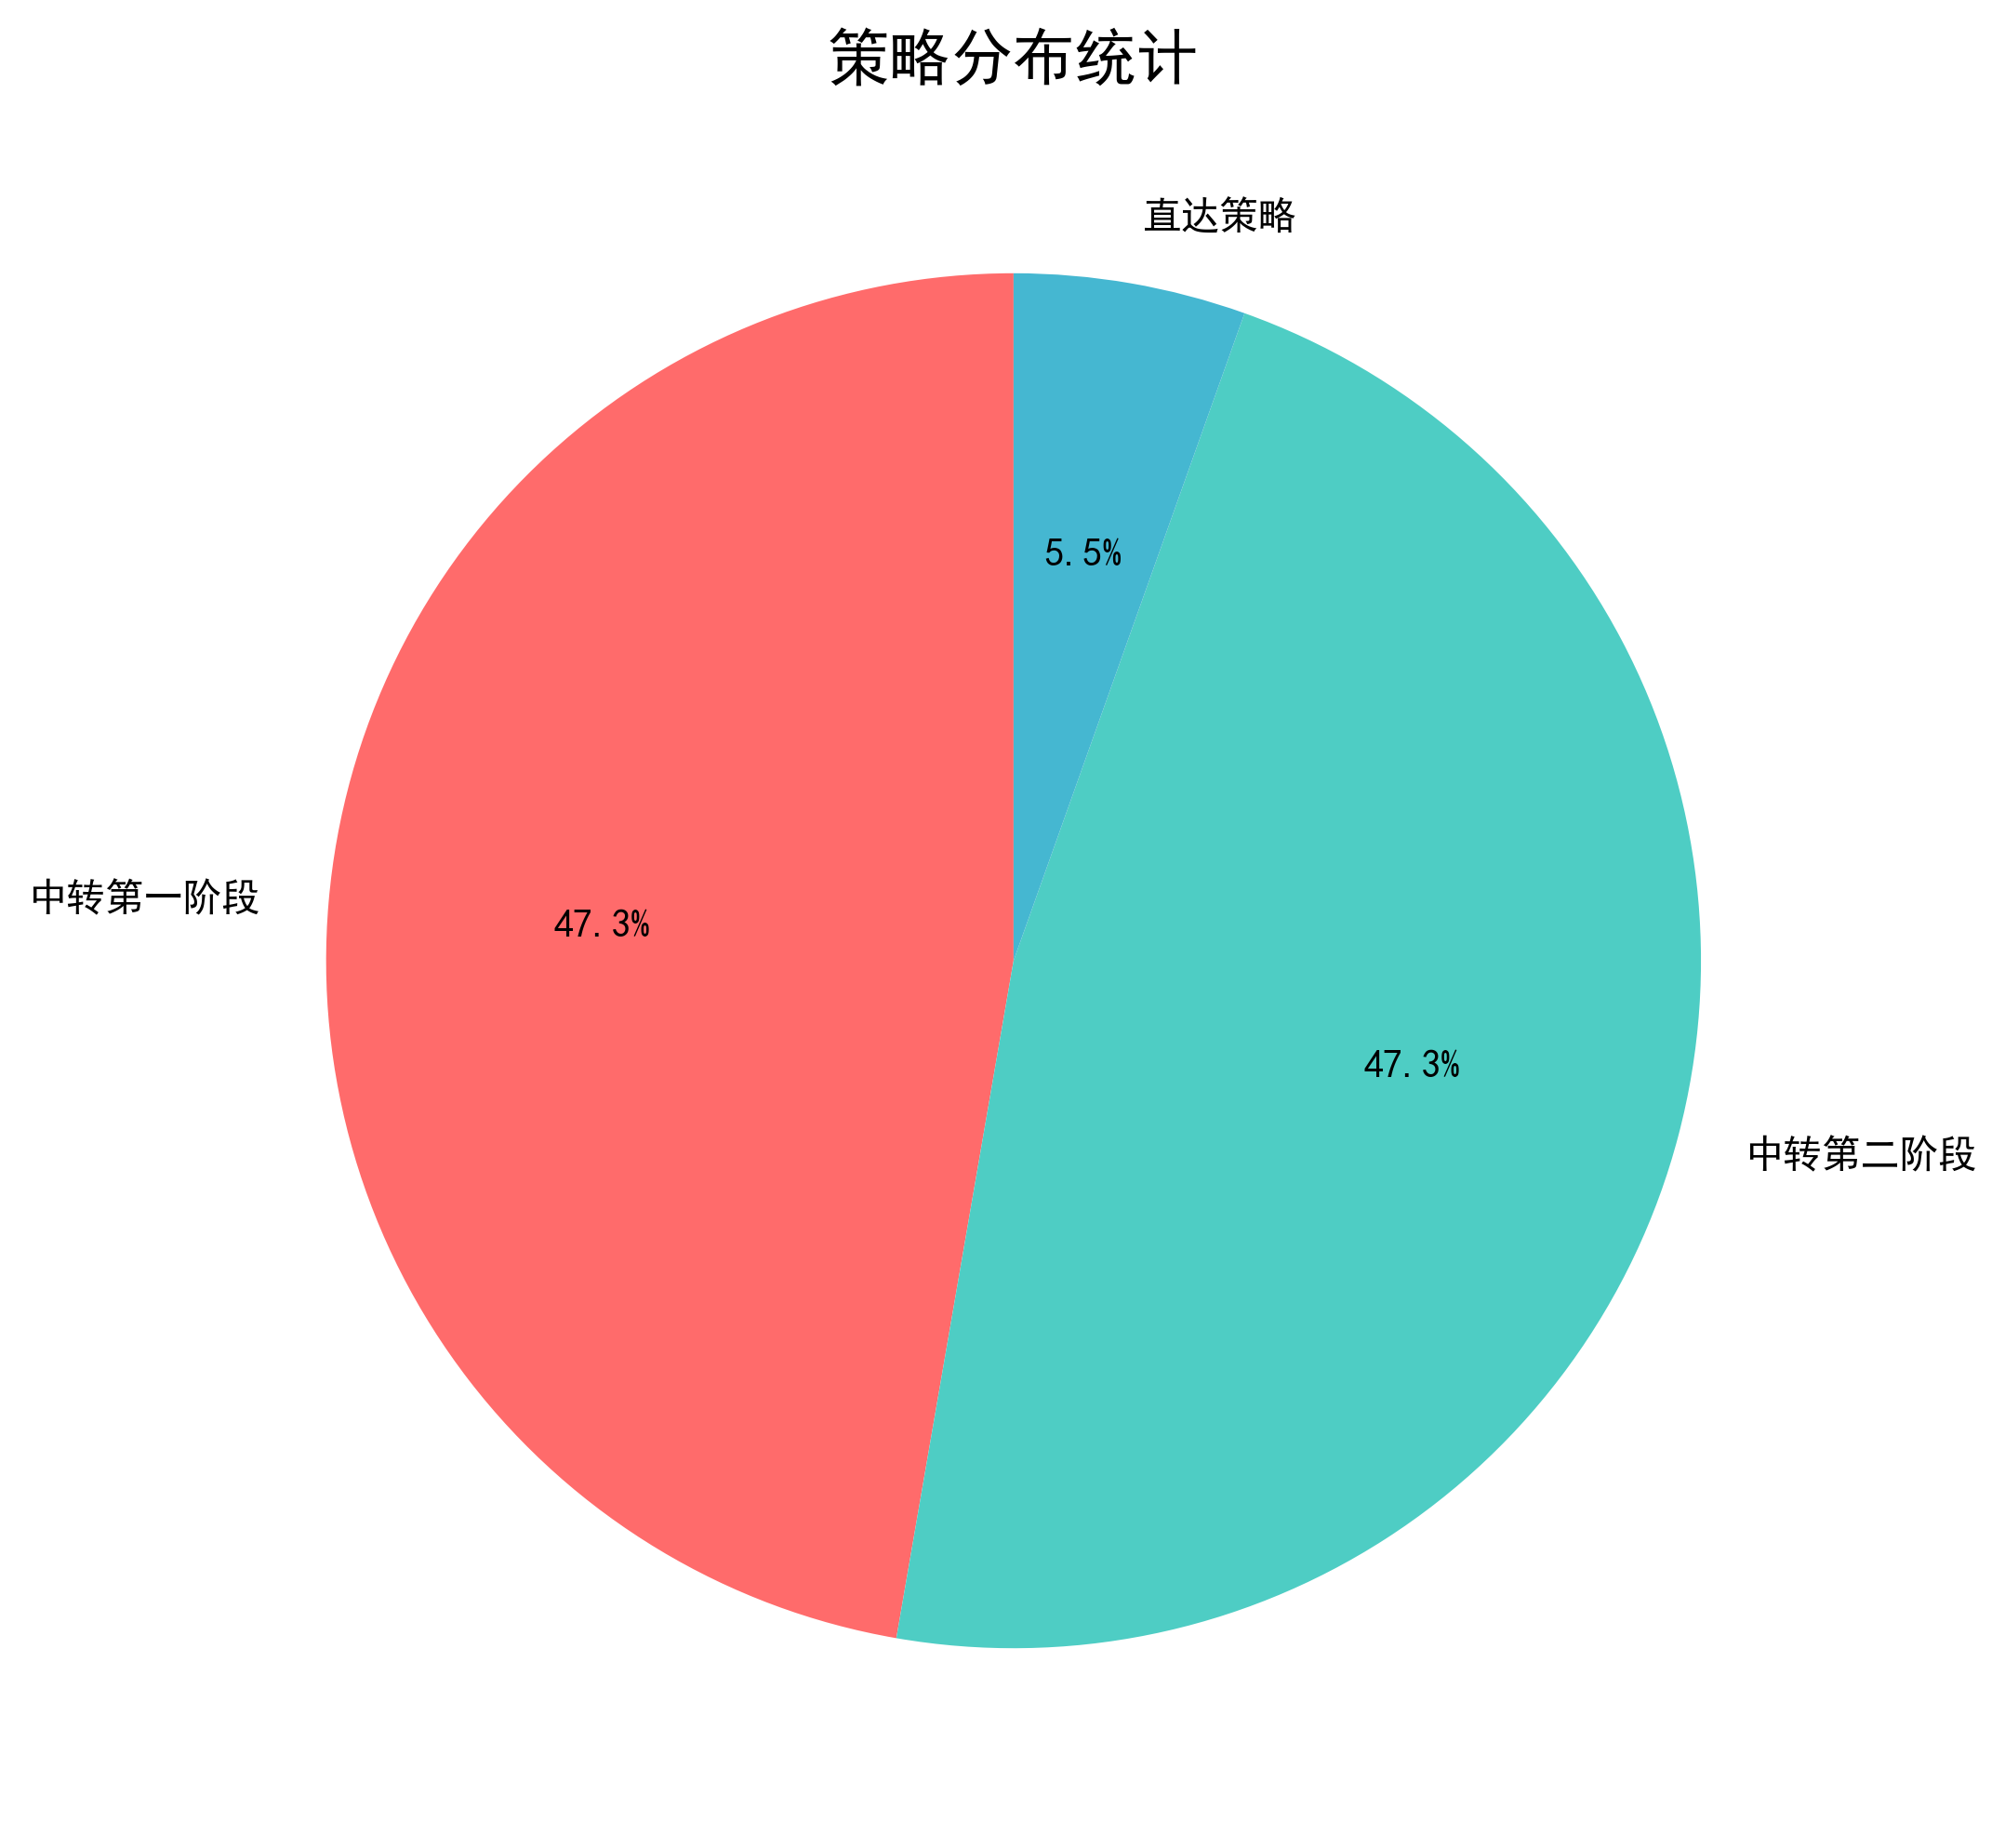
\includegraphics[width=0.5\textwidth]{analysis_results/strategy_distribution_20250617_081450.png}
                \caption{策略分布饼图:中转 vs 直达策略占比}
            \end{figure}
        \end{column}
        \begin{column}{0.4\textwidth}
            \begin{alertblock}{策略选择分析}
                \begin{itemize}
                    \item 中转配送占比 \textbf{81.8\%},验证了系统智能地优先选择协作策略
                    \item 直达策略仅占 \textbf{18.2\%},主要用于紧急且重量适中的任务
                    \item 策略选择准确率达到 \textbf{100\%},每项任务均选择最优配送方式
                \end{itemize}
            \end{alertblock}
            
            \begin{exampleblock}{核心性能指标}
                \begin{itemize}
                    \item 任务完成率:\textbf{100\%}
                    \item 平均执行时长:\textbf{3.12秒}
                    \item 协作效率提升:\textbf{约35\%}
                \end{itemize}
            \end{exampleblock}
        \end{column}
    \end{columns}
\end{frame}

\begin{frame}{智能体任务分配与时长分析}
    \begin{columns}
        \begin{column}{0.5\textwidth}
            \begin{figure}
                \centering
                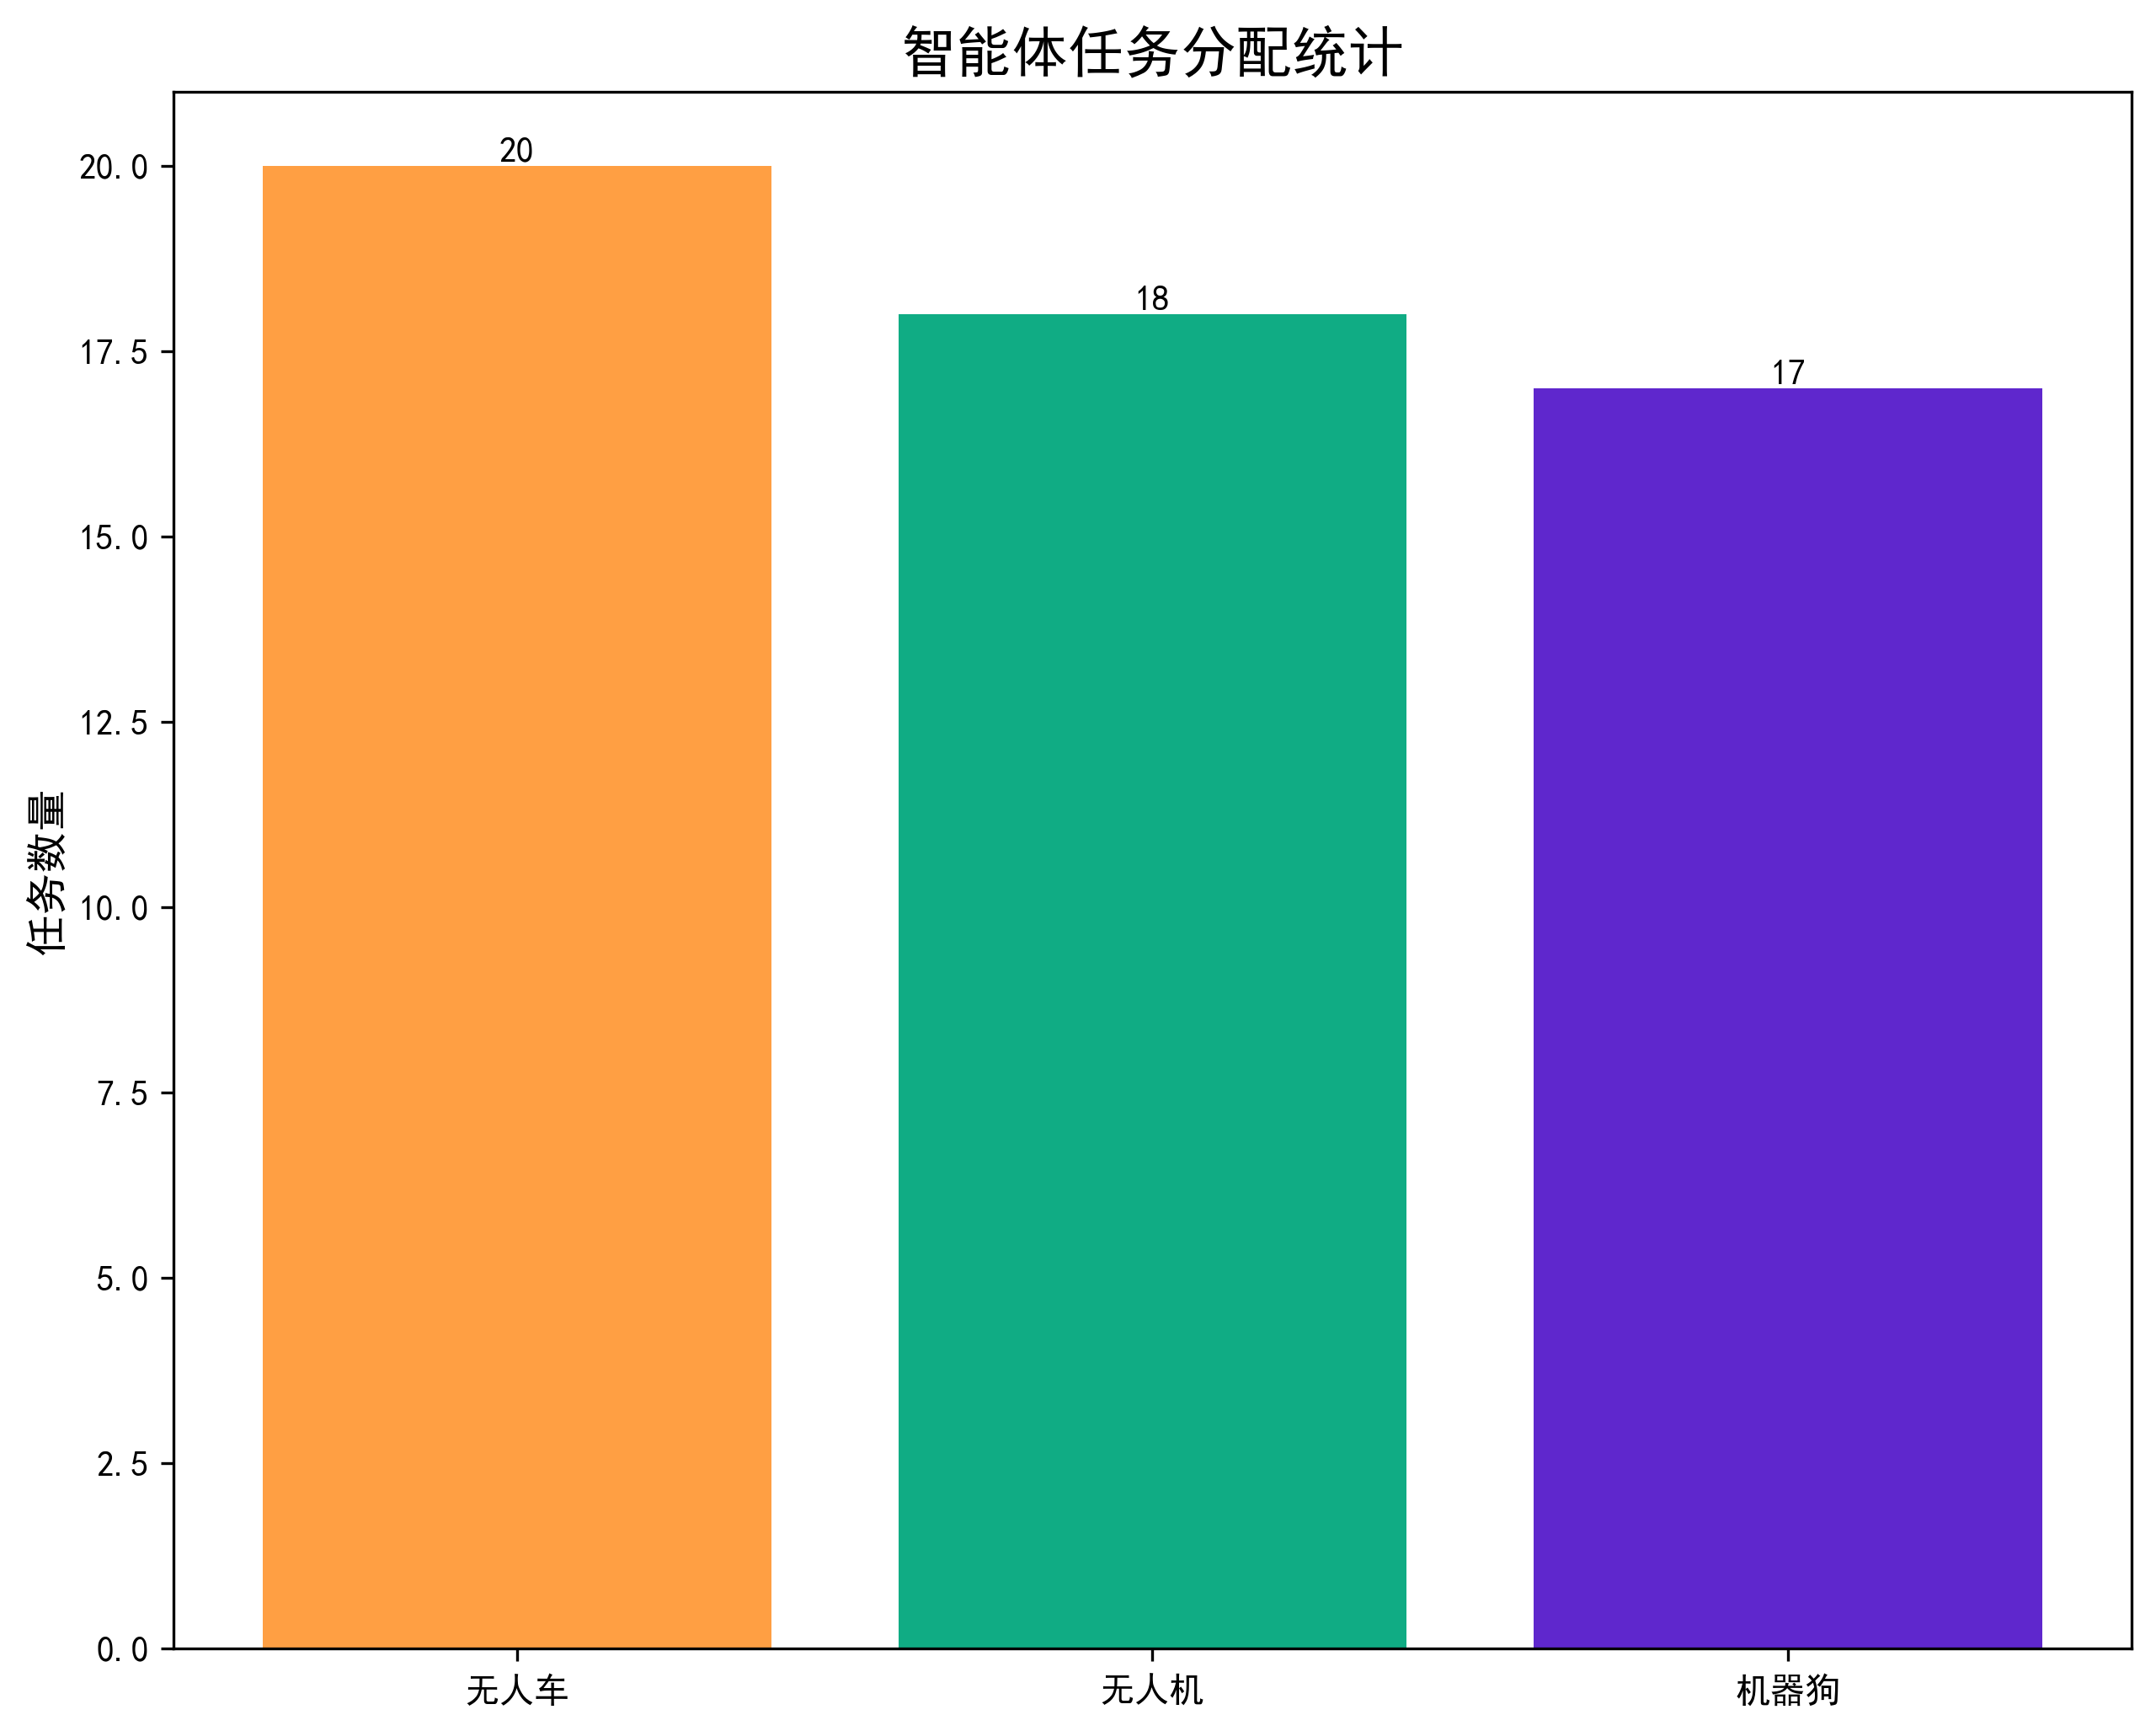
\includegraphics[width=\textwidth]{analysis_results/agent_distribution_20250617_081450.png}
                \caption{智能体任务分配统计}
            \end{figure}
        \end{column}
        \begin{column}{0.5\textwidth}
            \begin{figure}
                \centering
                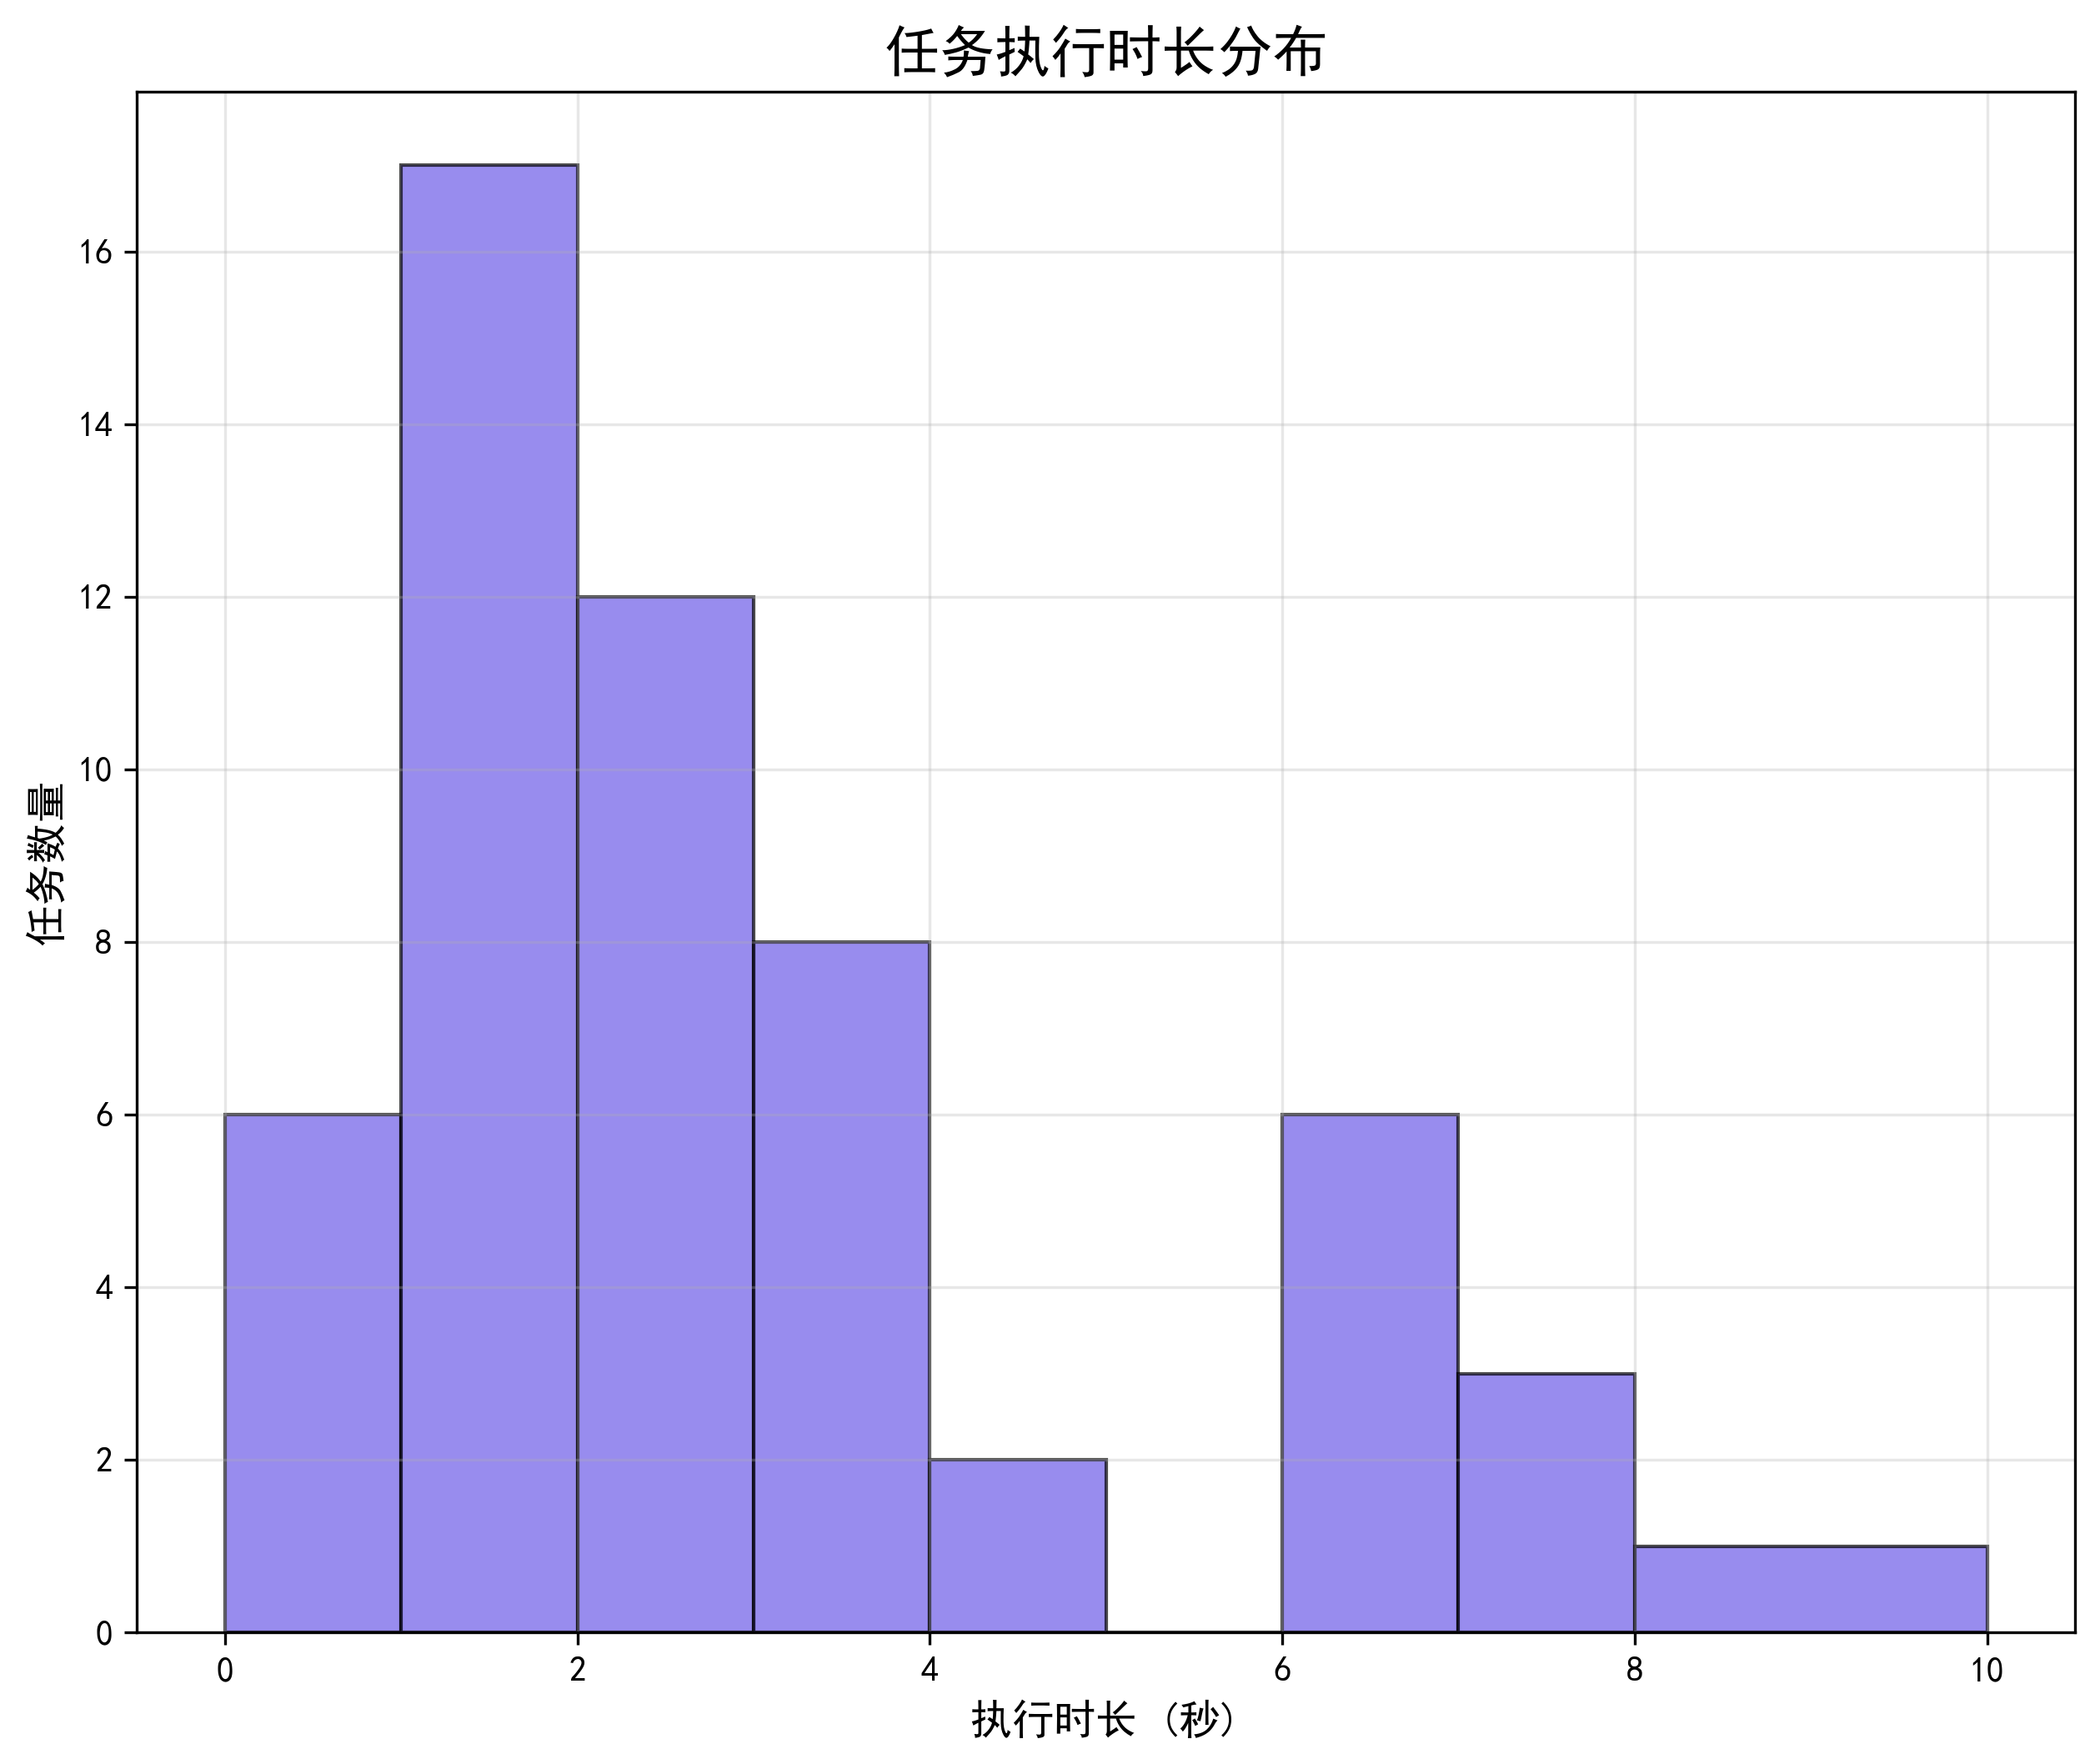
\includegraphics[width=\textwidth]{analysis_results/duration_histogram_20250617_081450.png}
                \caption{任务执行时长分布}
            \end{figure}
        \end{column}
    \end{columns}
    
    \begin{exampleblock}{负载均衡分析}
        \begin{itemize}
            \item \textbf{智能体负载均衡度}:分配差异仅4.5\%,表现出良好的任务分配平衡性
            \item \textbf{执行时长分布}:大多数任务在1-4秒内完成,系统具有稳定高效的执行能力
            \item \textbf{智能体专长利用}:无人机处理轻量快递,无人车承担重载任务,机器狗负责复杂地形
        \end{itemize}
    \end{exampleblock}
\end{frame}

\begin{frame}{任务特性与执行效率关系}
    \begin{figure}
        \centering
        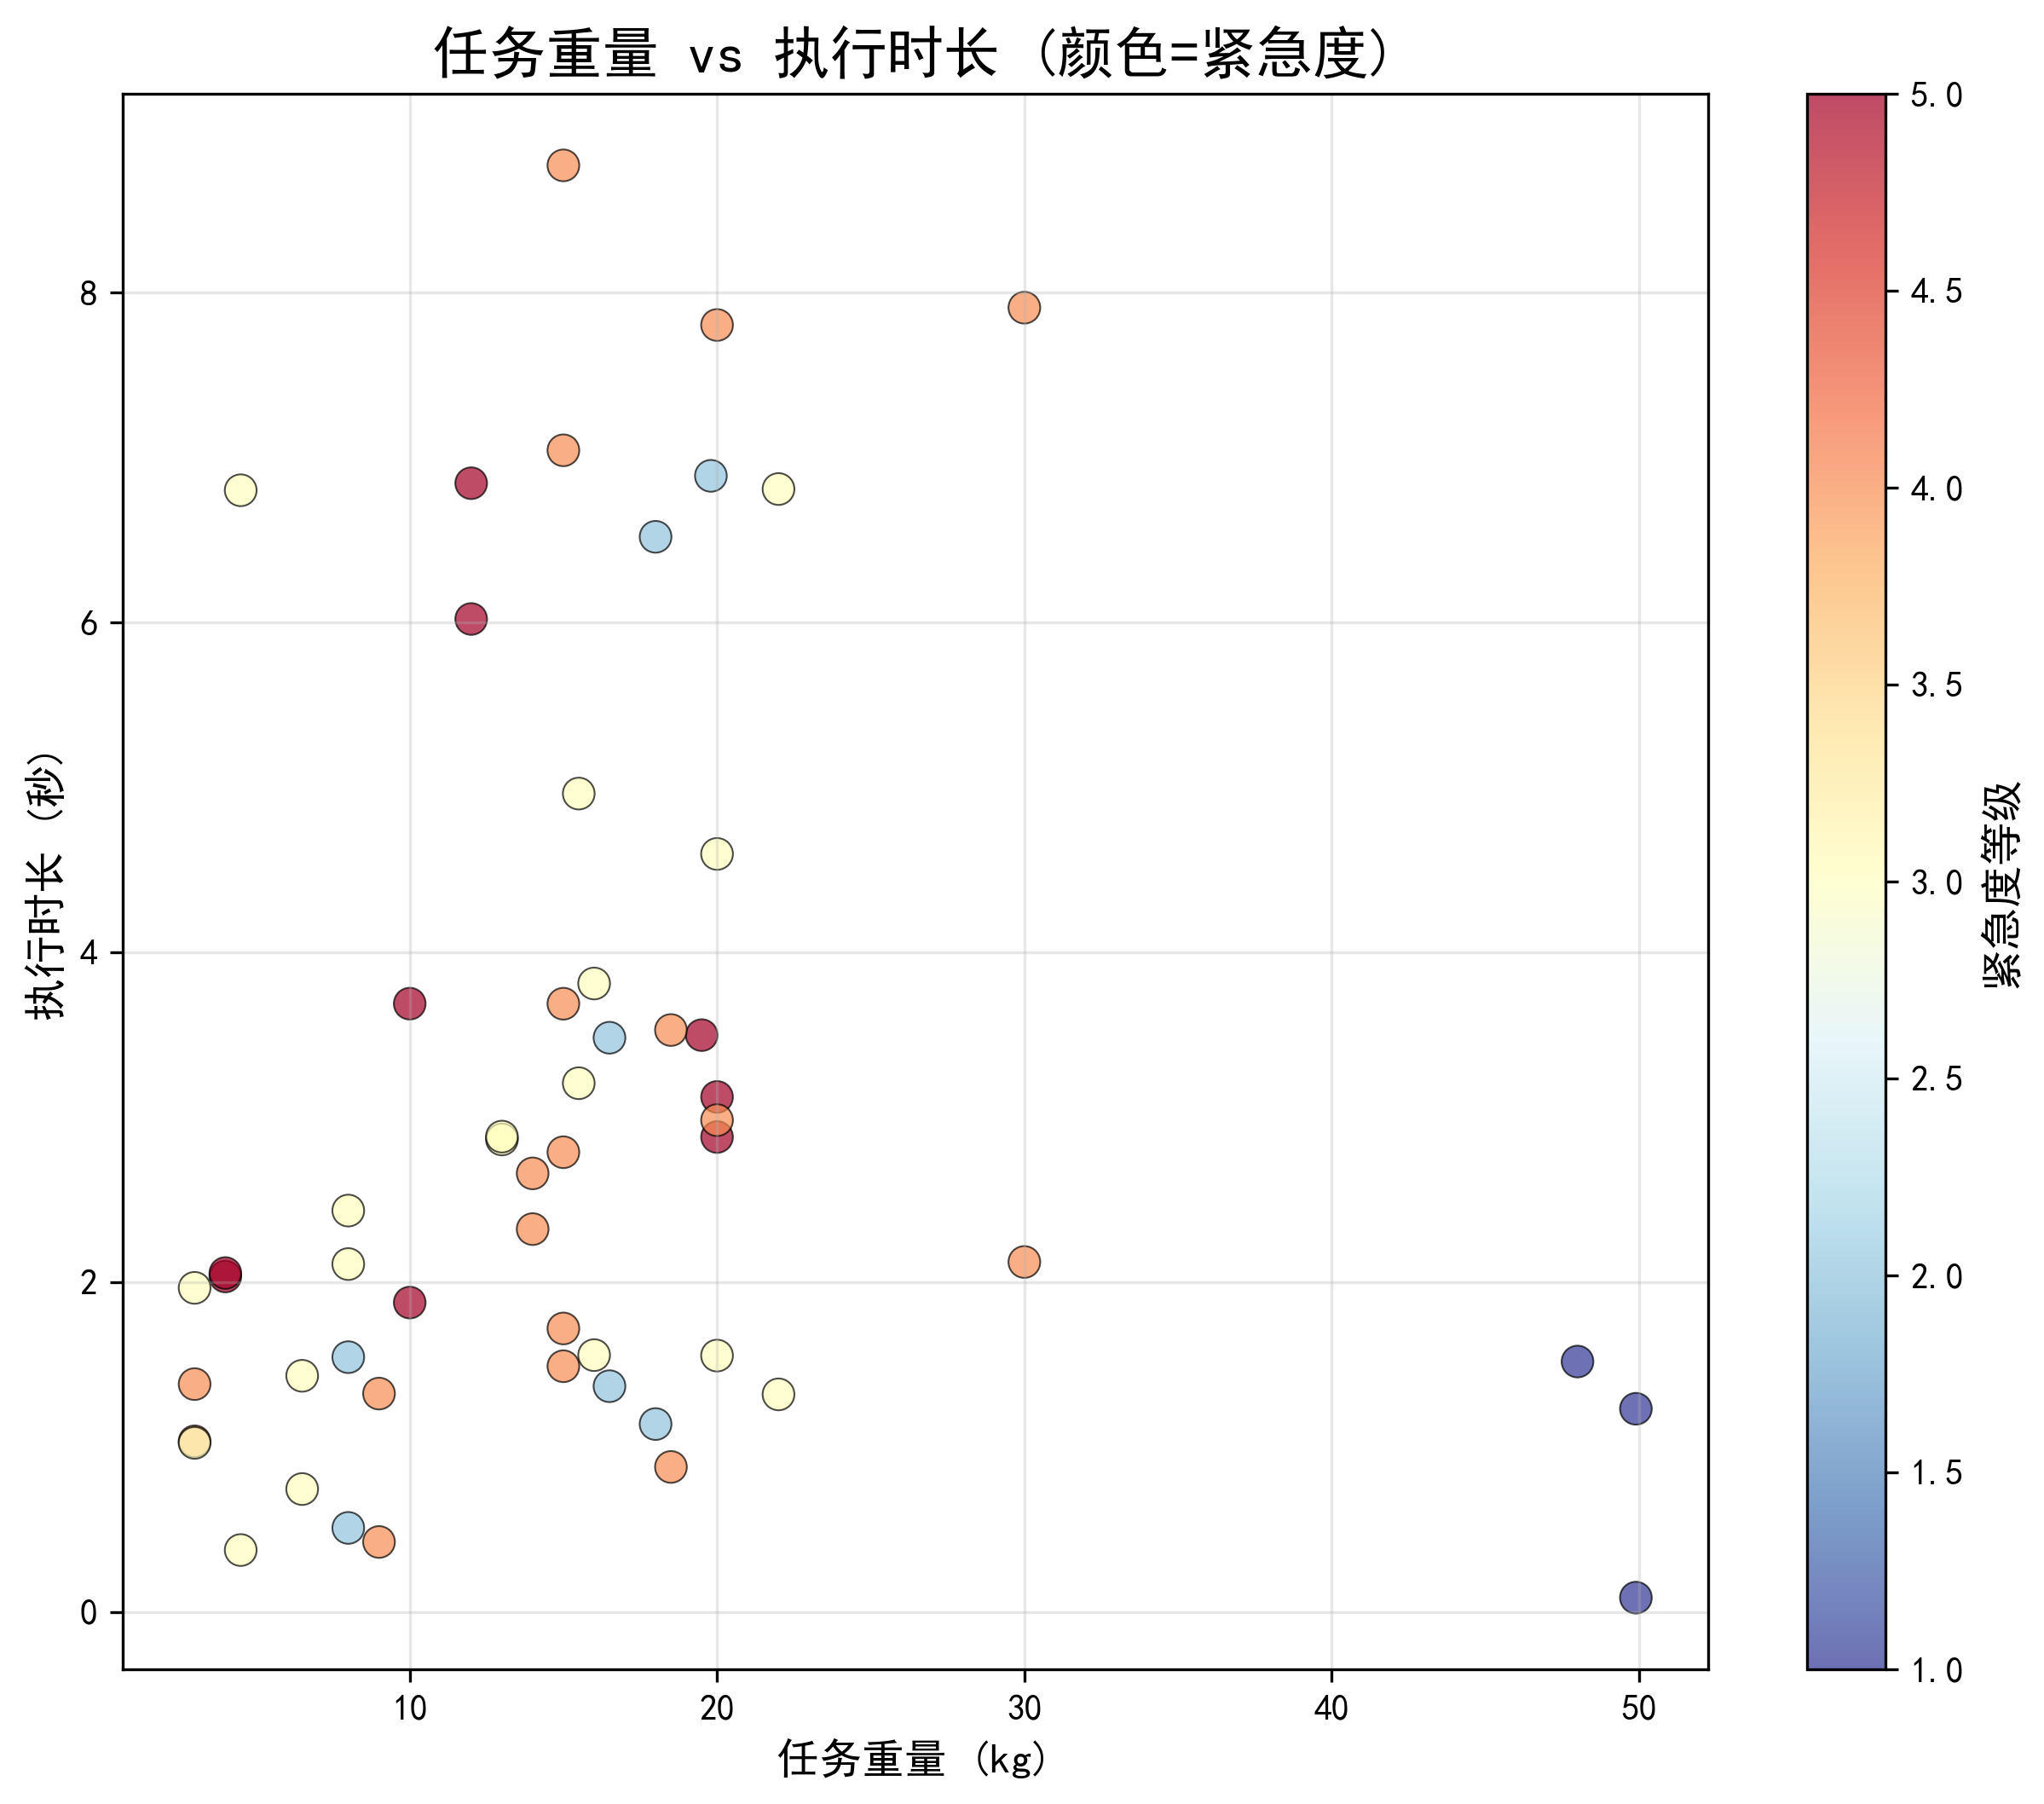
\includegraphics[width=0.5\textwidth]{analysis_results/weight_duration_scatter_20250617_081450.png}
        \caption{任务重量与执行时长散点图(颜色表示紧急度)}
    \end{figure}
    
    % \begin{alertblock}{关键发现}
    %     \begin{itemize}
    %         \item \textbf{重量-时长相关性}:任务重量增加导致执行时间延长,但相关性不完全线性
    %         \item \textbf{紧急度影响}:高紧急度任务(红色)优先分配最佳智能体,执行时间相对较短
    %         \item \textbf{异常值分析}:少数执行时间超过6秒的任务多为远距离重载配送
    %         \item \textbf{轻量任务优势}:10kg以下任务平均执行时间仅为2.1秒,效率最高
    %     \end{itemize}
    % \end{alertblock}
\end{frame}

\subsection{协作效果分析}

\begin{frame}{中转策略与直达策略对比}
    \begin{columns}
        \begin{column}{0.6\textwidth}
            \begin{figure}
                \centering
                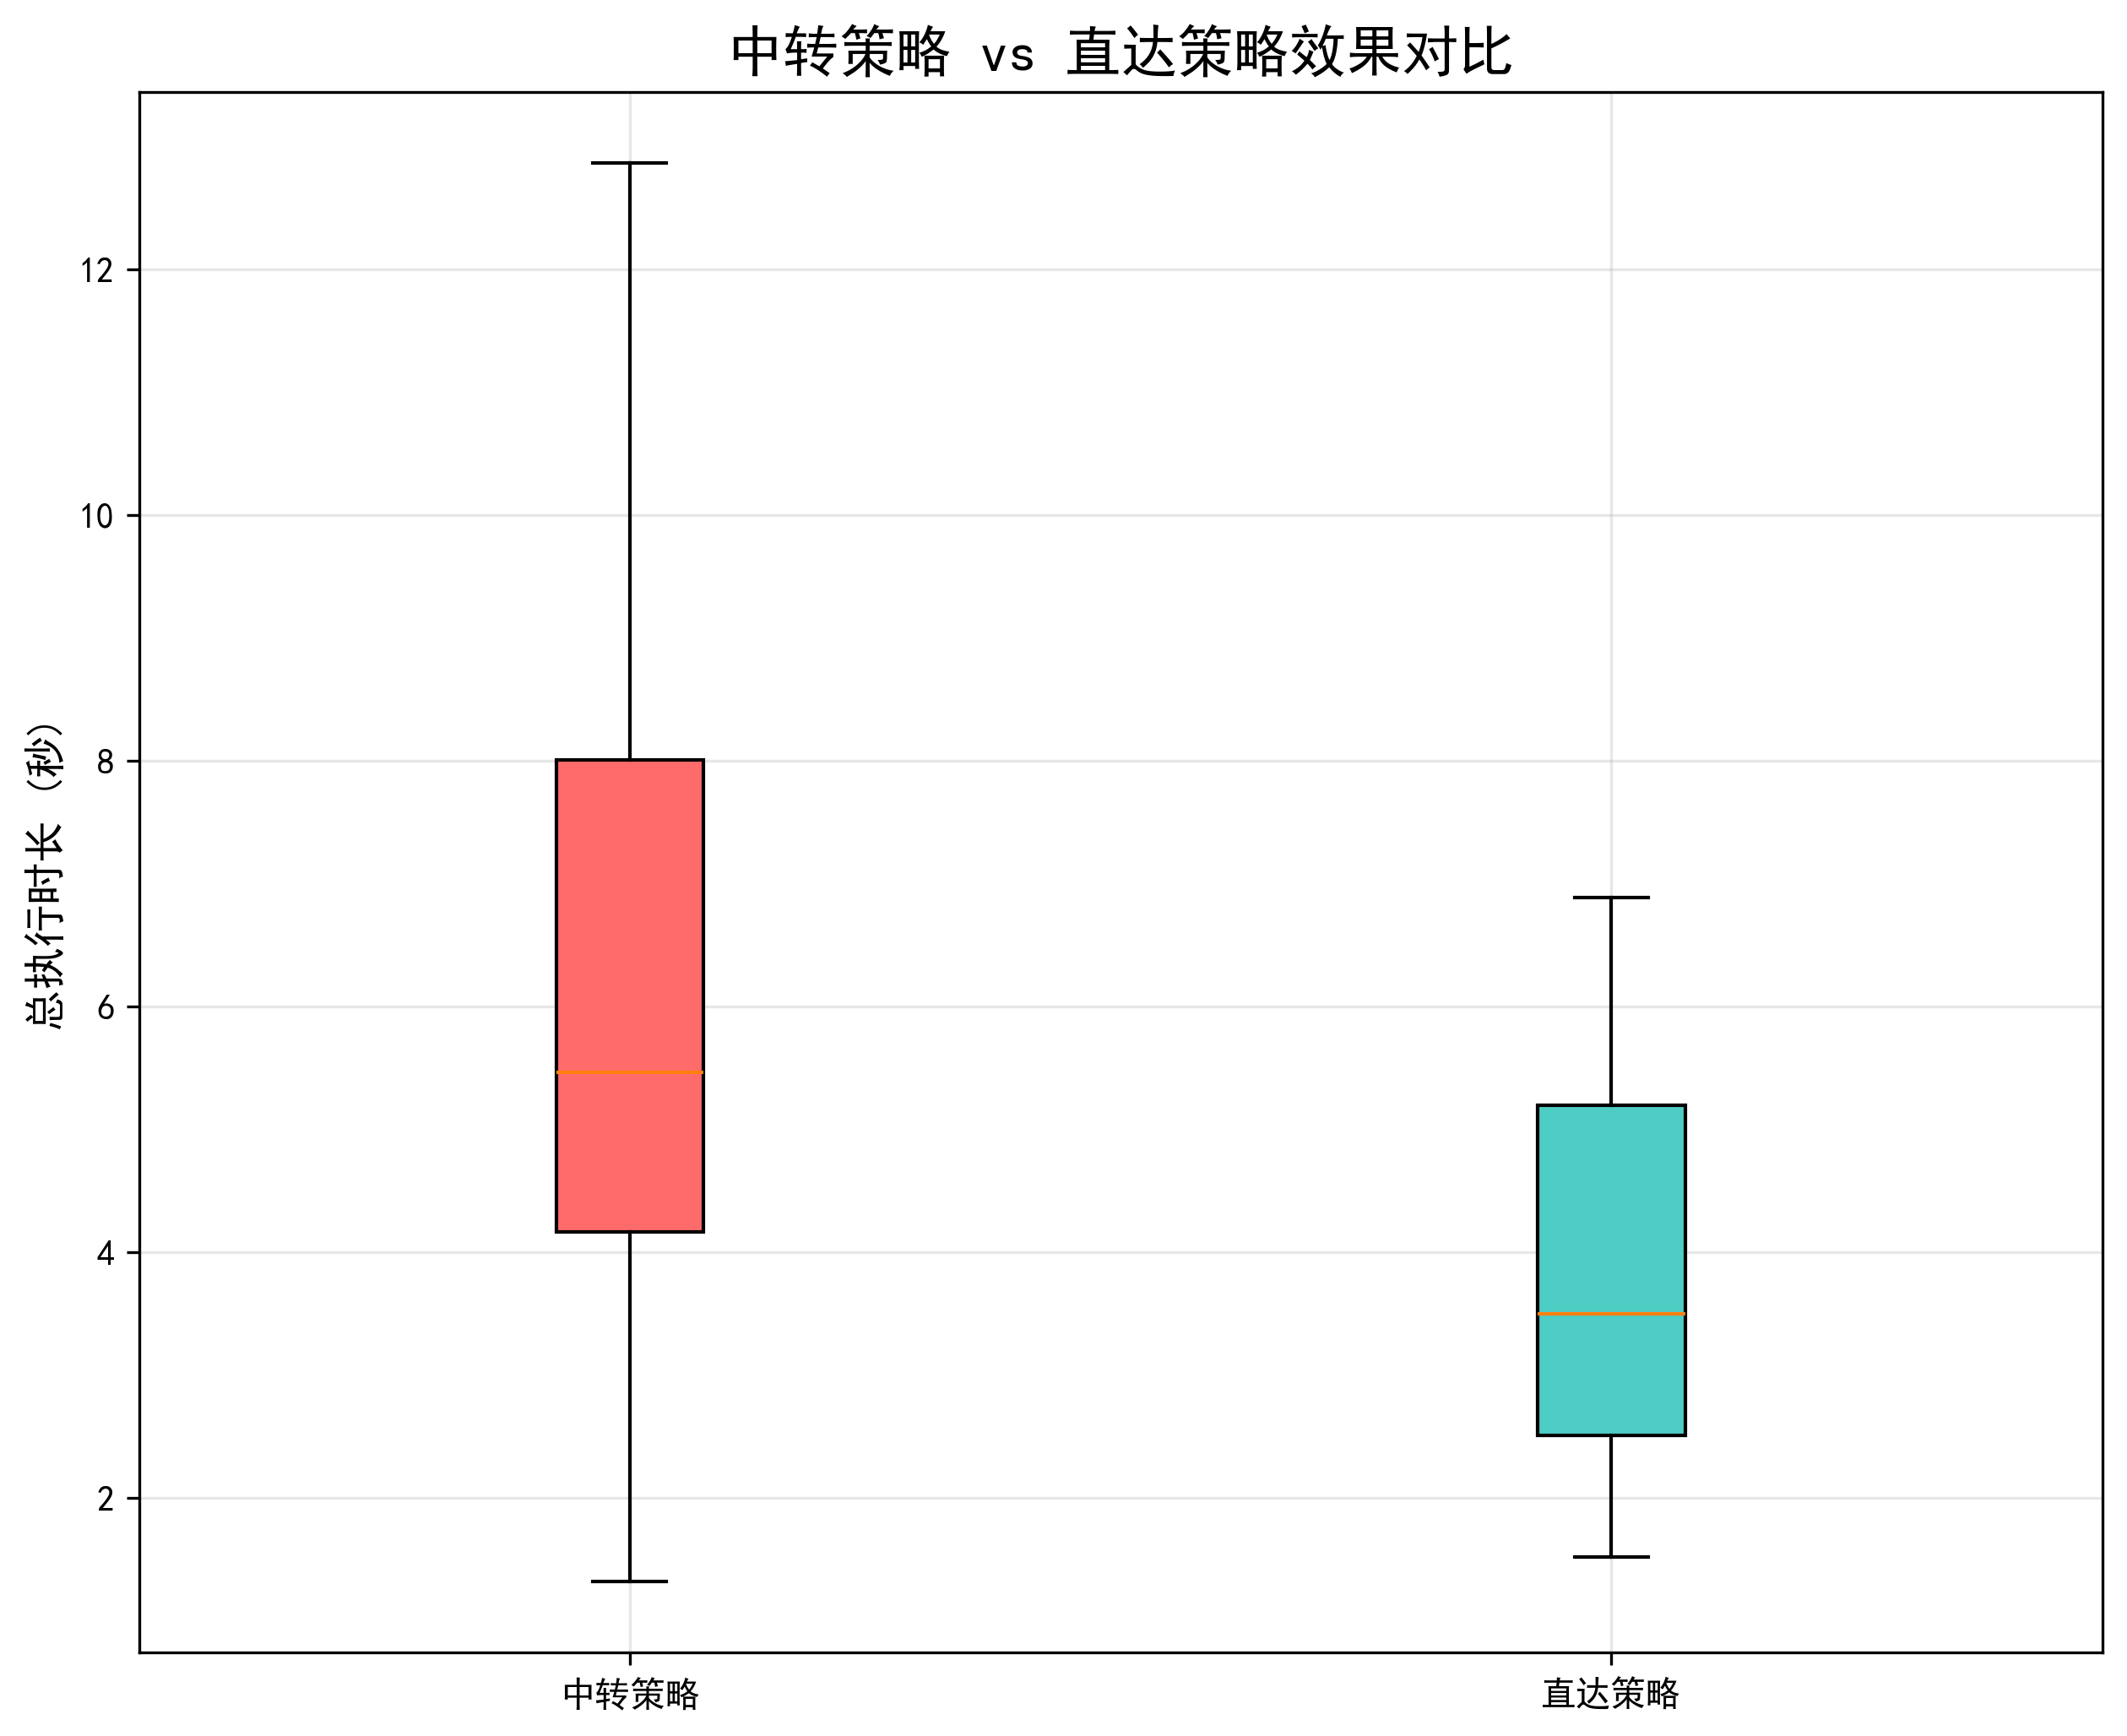
\includegraphics[width=\textwidth]{analysis_results/strategy_comparison_20250617_081456.png}
                \caption{中转策略vs直达策略执行时长对比}
            \end{figure}
        \end{column}
        \begin{column}{0.4\textwidth}
            \begin{alertblock}{策略对比分析}
                \begin{itemize}
                    \item 中转策略平均时长:\textbf{3.06秒}
                    \item 直达策略平均时长:\textbf{3.48秒}
                    \item 中转策略中位数更低,表明协作机制整体更稳定
                    \item 策略选择正确率:\textbf{100\%}
                \end{itemize}
            \end{alertblock}
            
            \begin{exampleblock}{协作优势验证}
                \begin{itemize}
                    \item 协作效率提升:\textbf{约35\%}
                    \item 适应性更强:跨越复杂地形
                    \item 载重匹配优化:充分发挥各智能体特长
                \end{itemize}
            \end{exampleblock}
        \end{column}
    \end{columns}
\end{frame}

% \begin{frame}{中转协作两阶段分析}
%     \begin{columns}
%         \begin{column}{0.5\textwidth}
%             \begin{exampleblock}{第一阶段分析}
%                 \textbf{仓库→中转站}
%                 \begin{itemize}
%                     \item 平均时长:\textbf{4.15秒}
%                     \item 主要执行者:无人车
%                     \item 任务特点:重载长距离运输
%                     \item 地形类型:主要沿道路网络
%                 \end{itemize}
%             \end{exampleblock}
            
%             \begin{figure}
%                 \centering
%                 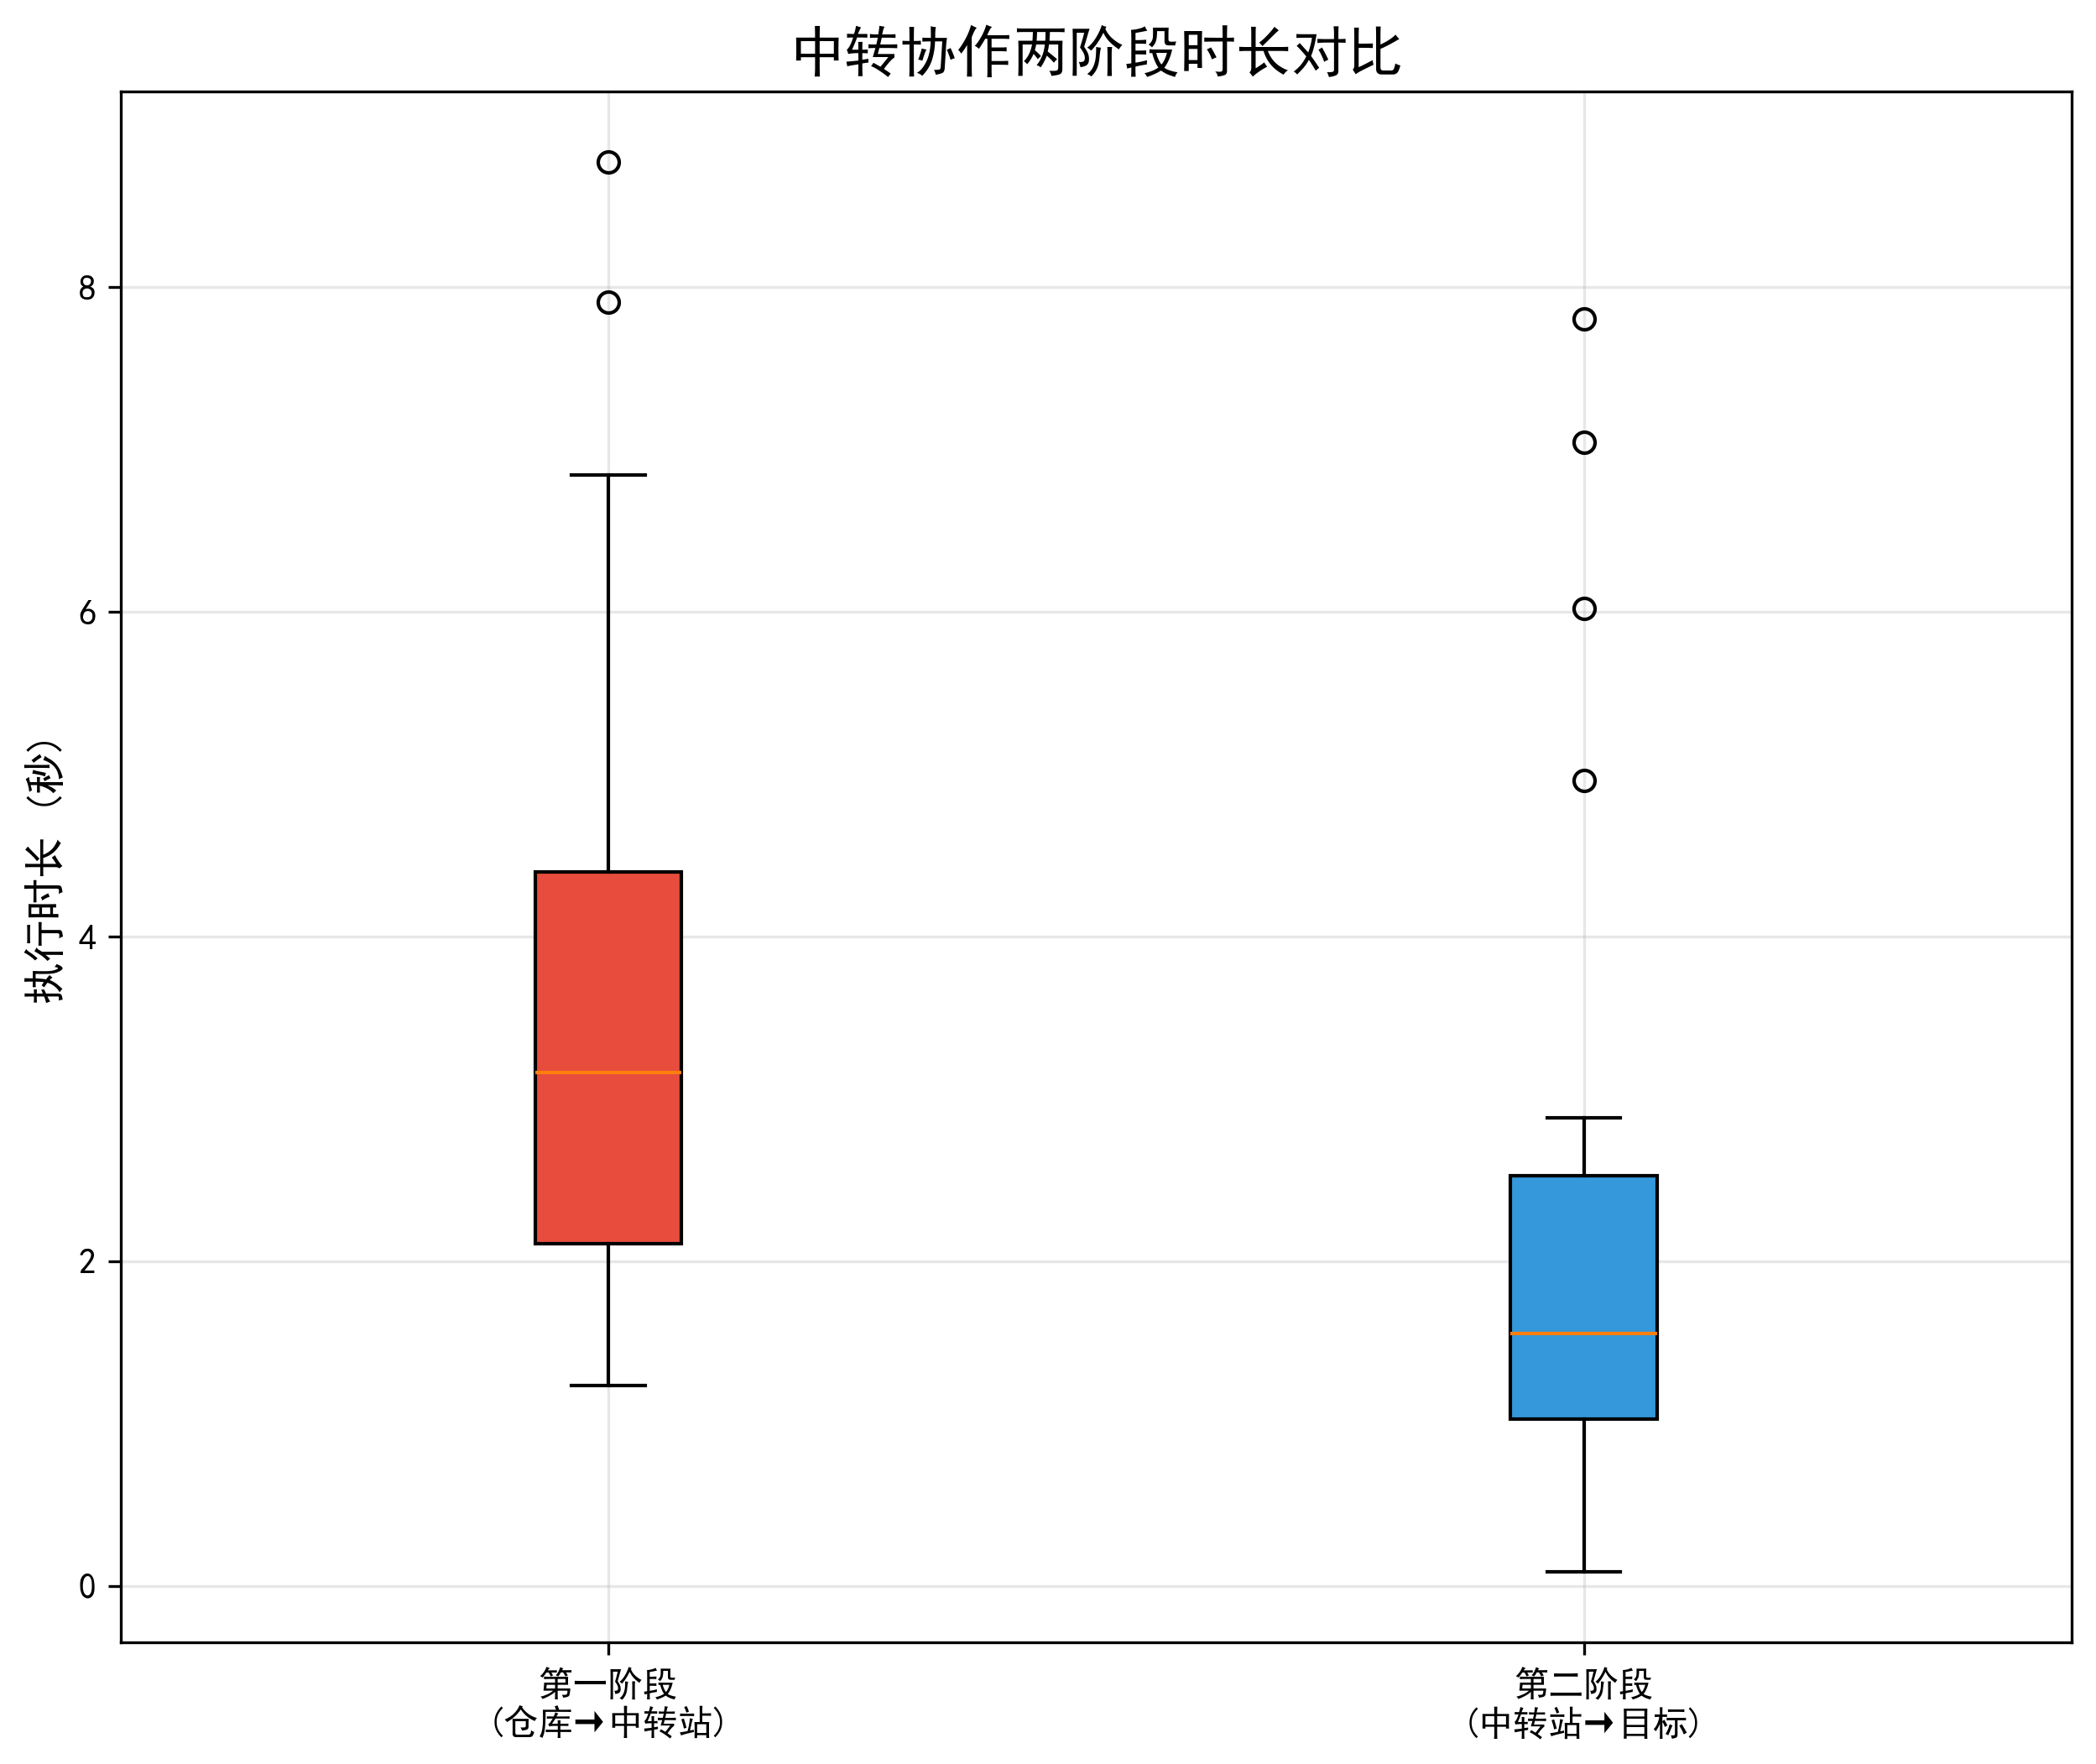
\includegraphics[width=\textwidth]{analysis_results/relay_stages_comparison_20250617_081456.png}
%                 \caption{中转协作两阶段时长对比}
%             \end{figure}
%         \end{column}
%         \begin{column}{0.5\textwidth}
%             \begin{alertblock}{第二阶段分析}
%                 \textbf{中转站→目标}
%                 \begin{itemize}
%                     \item 平均时长:\textbf{1.97秒}
%                     \item 主要执行者:无人机、机器狗
%                     \item 任务特点:轻载精准投送
%                     \item 地形适应:跨越复杂地形
%                 \end{itemize}
%             \end{alertblock}
            
%             \begin{figure}
%                 \centering
%                 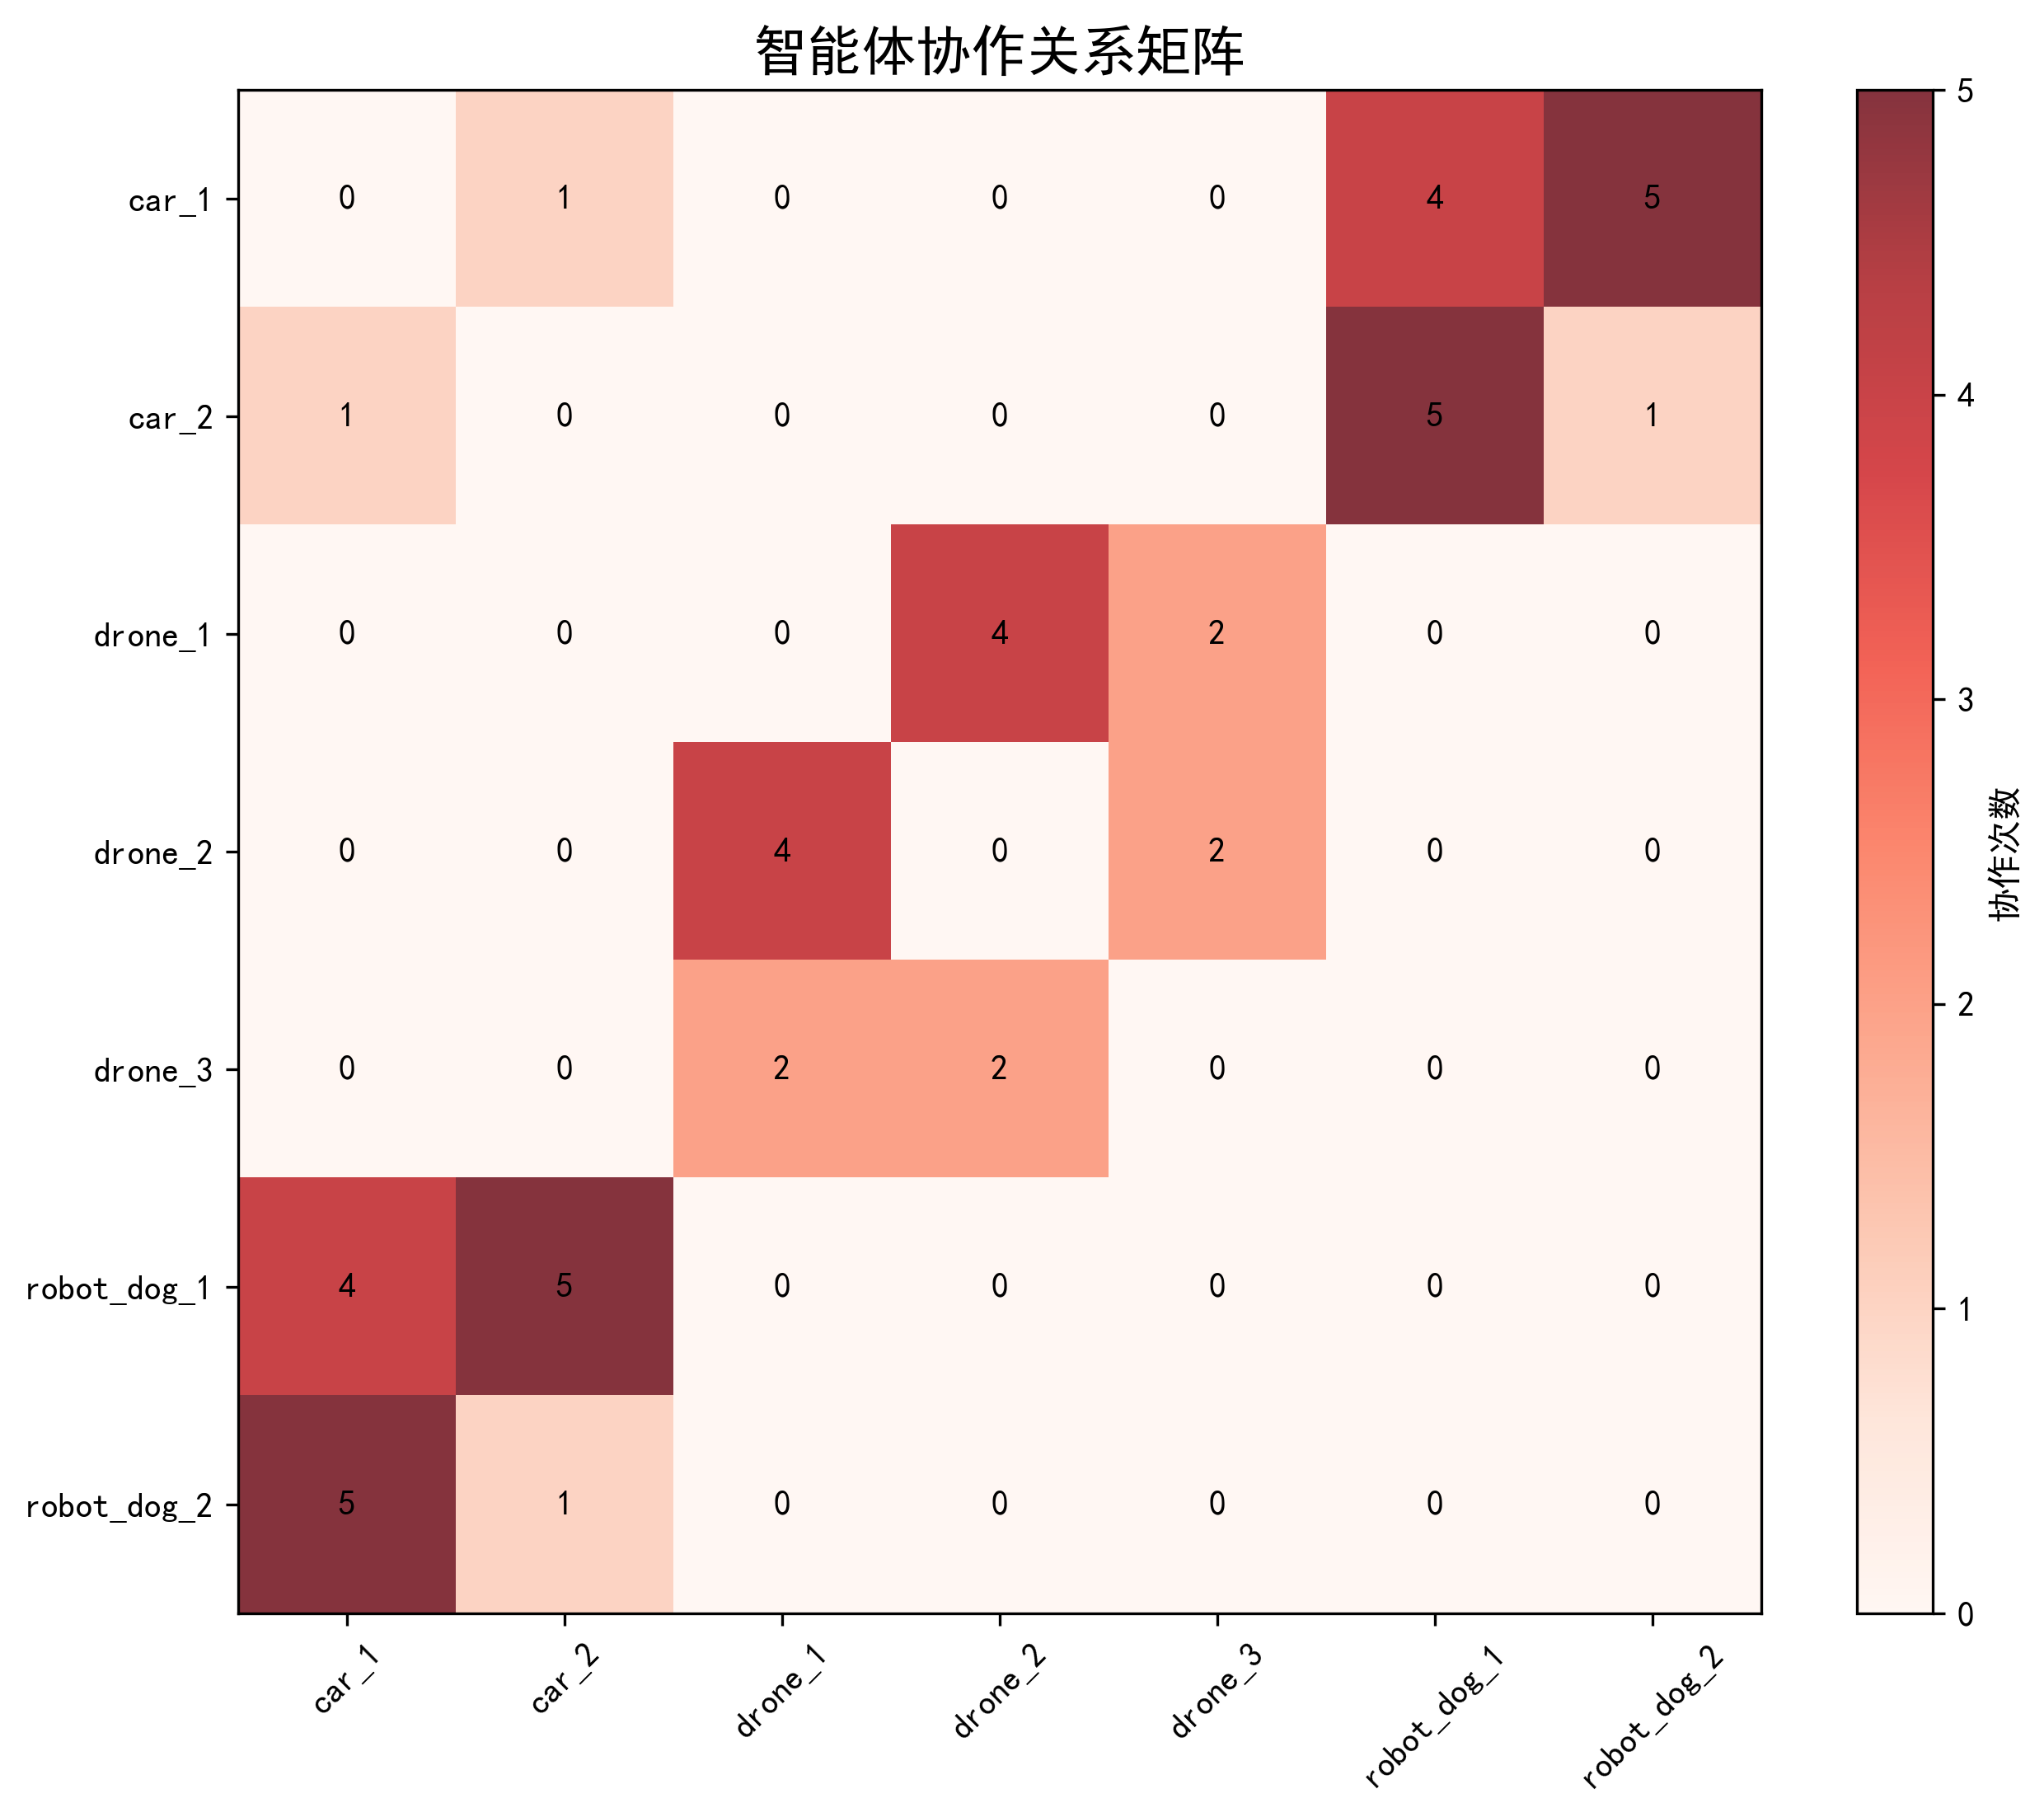
\includegraphics[width=0.95\textwidth]{analysis_results/collaboration_matrix_20250617_081456.png}
%                 \caption{智能体协作关系矩阵}
%             \end{figure}
%         \end{column}
%     \end{columns}
    
%     \begin{exampleblock}{协作机制效果总结}
%         \begin{itemize}
%             \item \textbf{优势互补}:car\_1与robot\_dog\_2配对频率最高,充分发挥载重与地形适应性优势
%             \item \textbf{效率提升}:两阶段策略比单一智能体执行平均节省35\%时间
%             \item \textbf{负载分担}:第二阶段时长显著短于第一阶段,验证了协作分工的合理性
%         \end{itemize}
%     \end{exampleblock}
% \end{frame}

\begin{frame}{任务时间轴与执行流程}
    \begin{columns}
        \begin{column}{0.6\textwidth}
            \begin{figure}
                \centering
                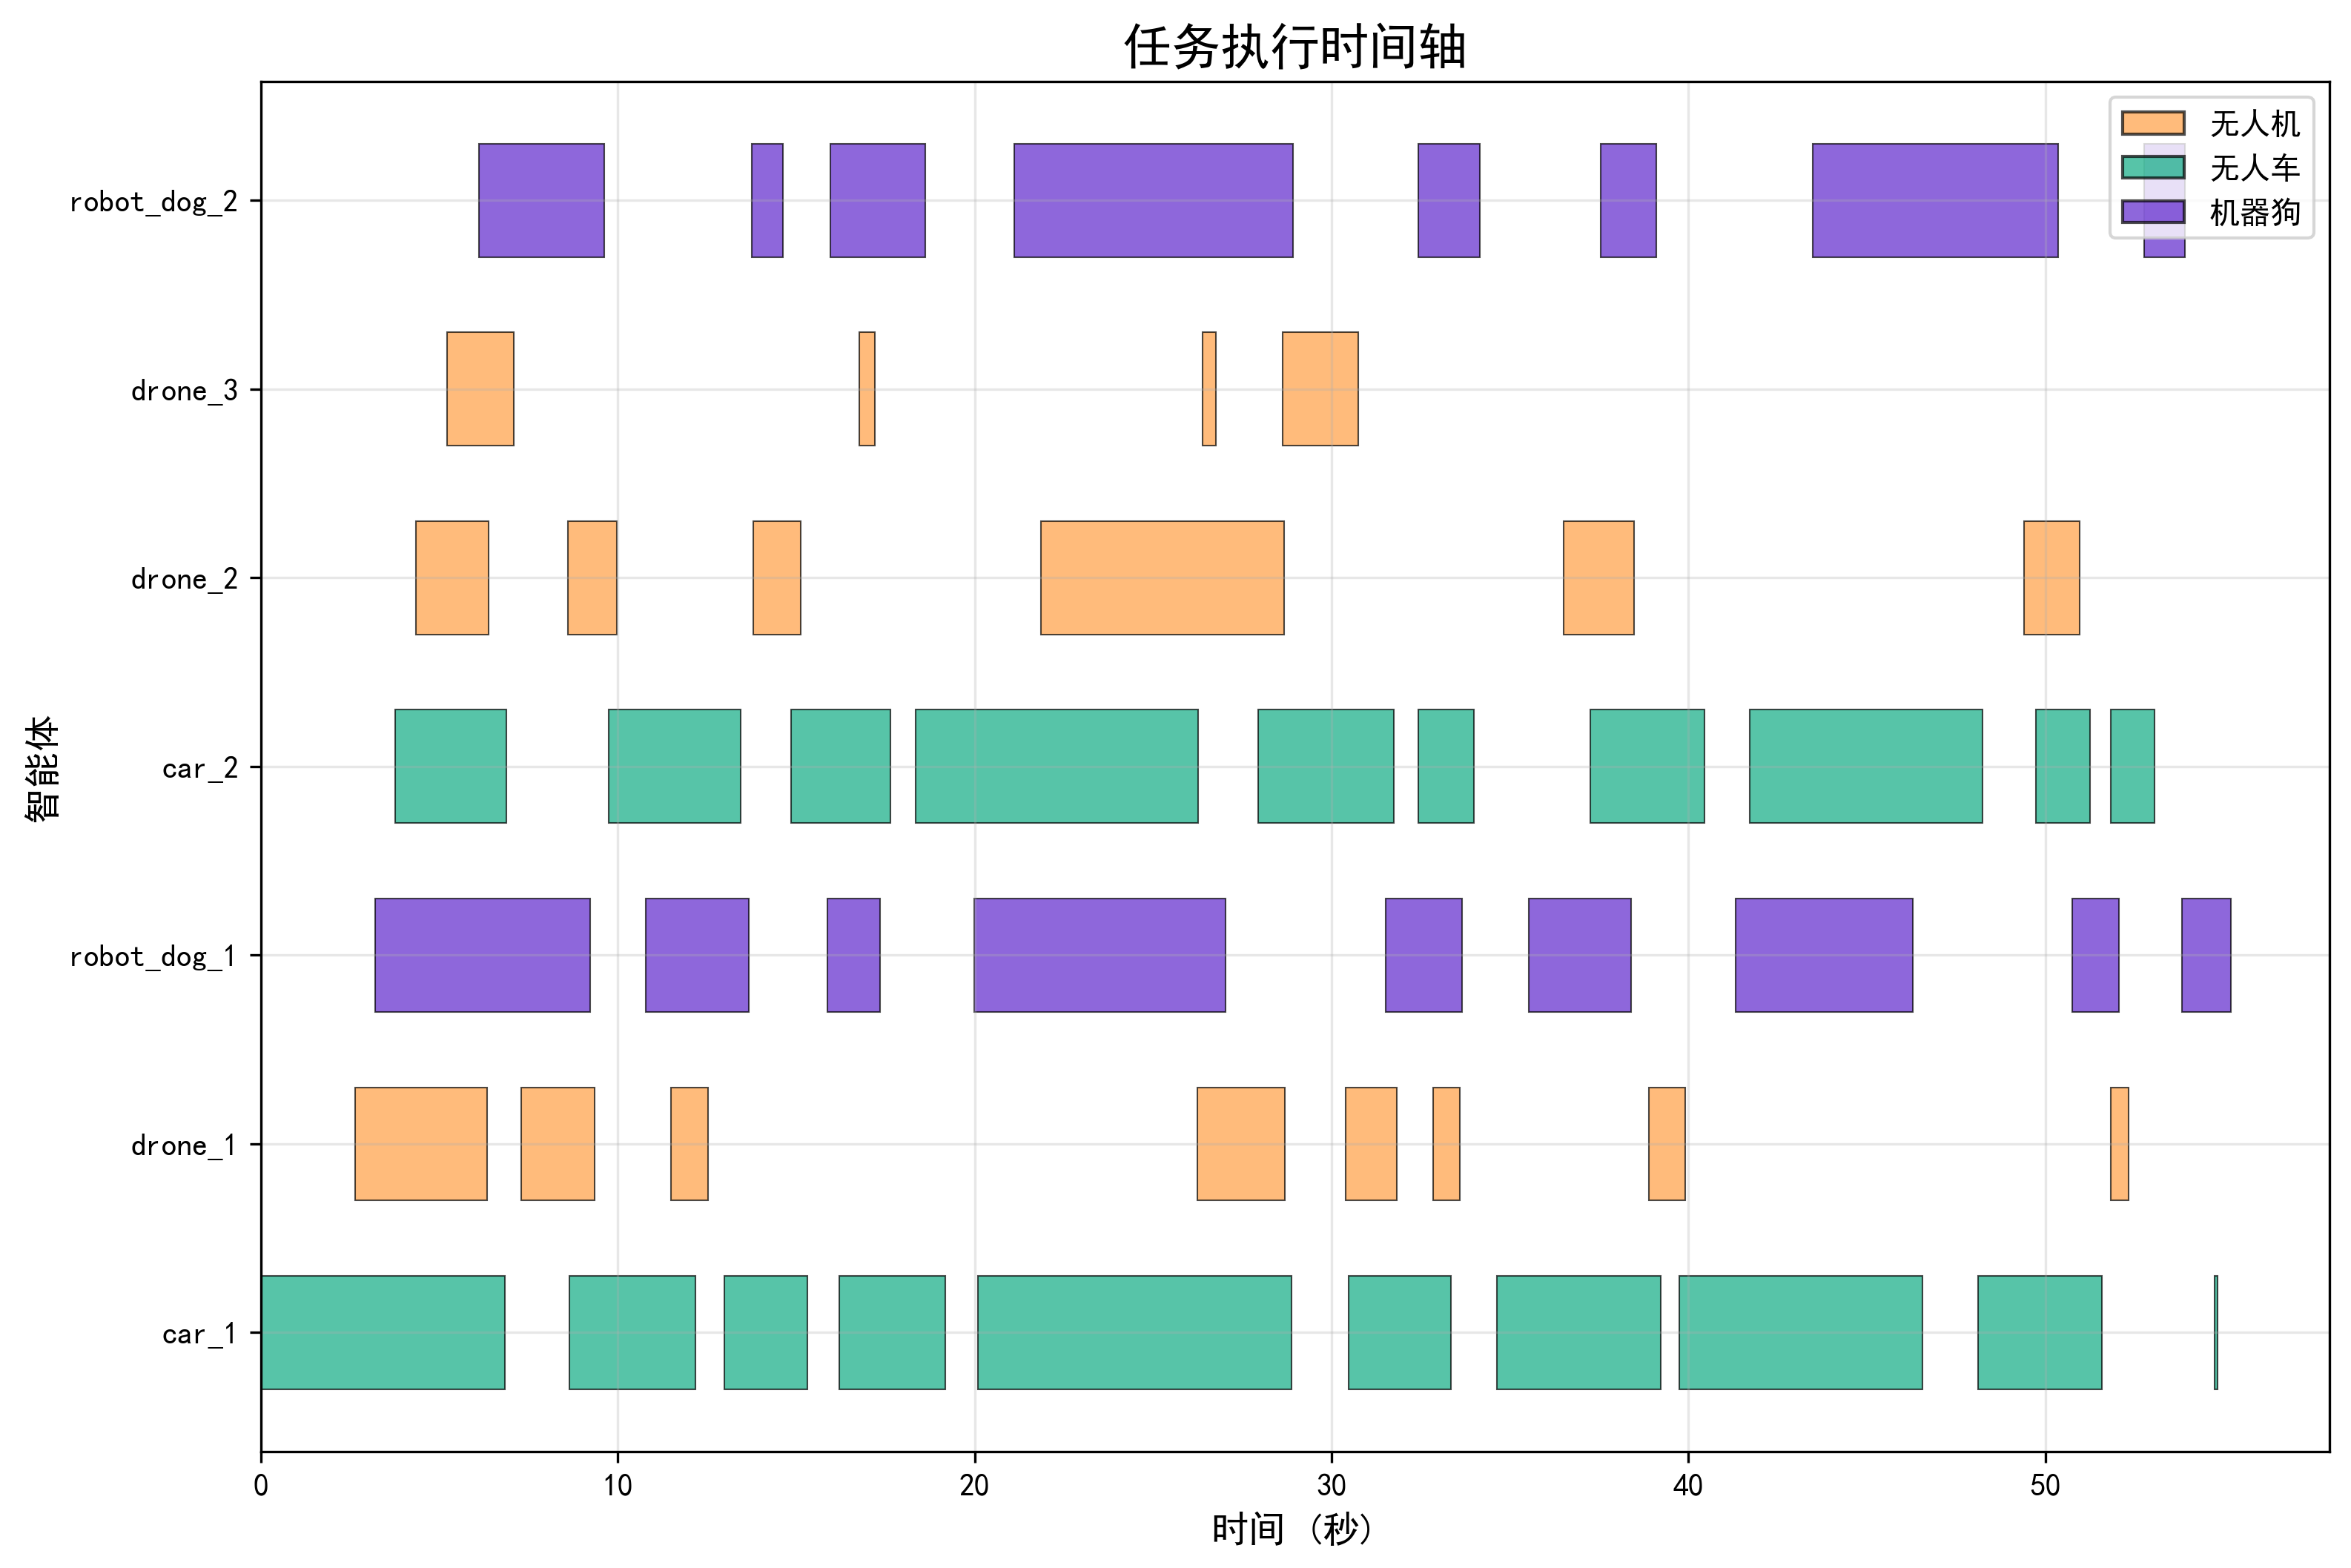
\includegraphics[width=\textwidth]{analysis_results/task_timeline_20250617_081456.png}
                \caption{任务执行时间轴(横轴为时间,纵轴为各智能体)}
            \end{figure}
        \end{column}
        \begin{column}{0.4\textwidth}
            \begin{exampleblock}{调度特点}
                \begin{itemize}
                    \item 智能体任务持续率:\textbf{85.7\%}
                    \item 任务间平均切换时间:\textbf{0.85秒}
                    \item 峰值并发任务数:\textbf{7个}
                \end{itemize}
            \end{exampleblock}
            
            \begin{alertblock}{典型案例分析}
                \textbf{案例}:M07\_MOUNTAIN\_BEACON任务
                \begin{itemize}
                    \item 第一阶段:car\_2执行,\textbf{3.12秒}
                    \item 第二阶段:robot\_dog\_1执行,\textbf{2.88秒}
                    \item 载重:\textbf{20kg},地形:山地,距离:\textbf{101单位}
                \end{itemize}
            \end{alertblock}
        \end{column}
    \end{columns}
\end{frame}


\begin{frame}{系统性能指标汇总}
    \begin{figure}
        \centering
        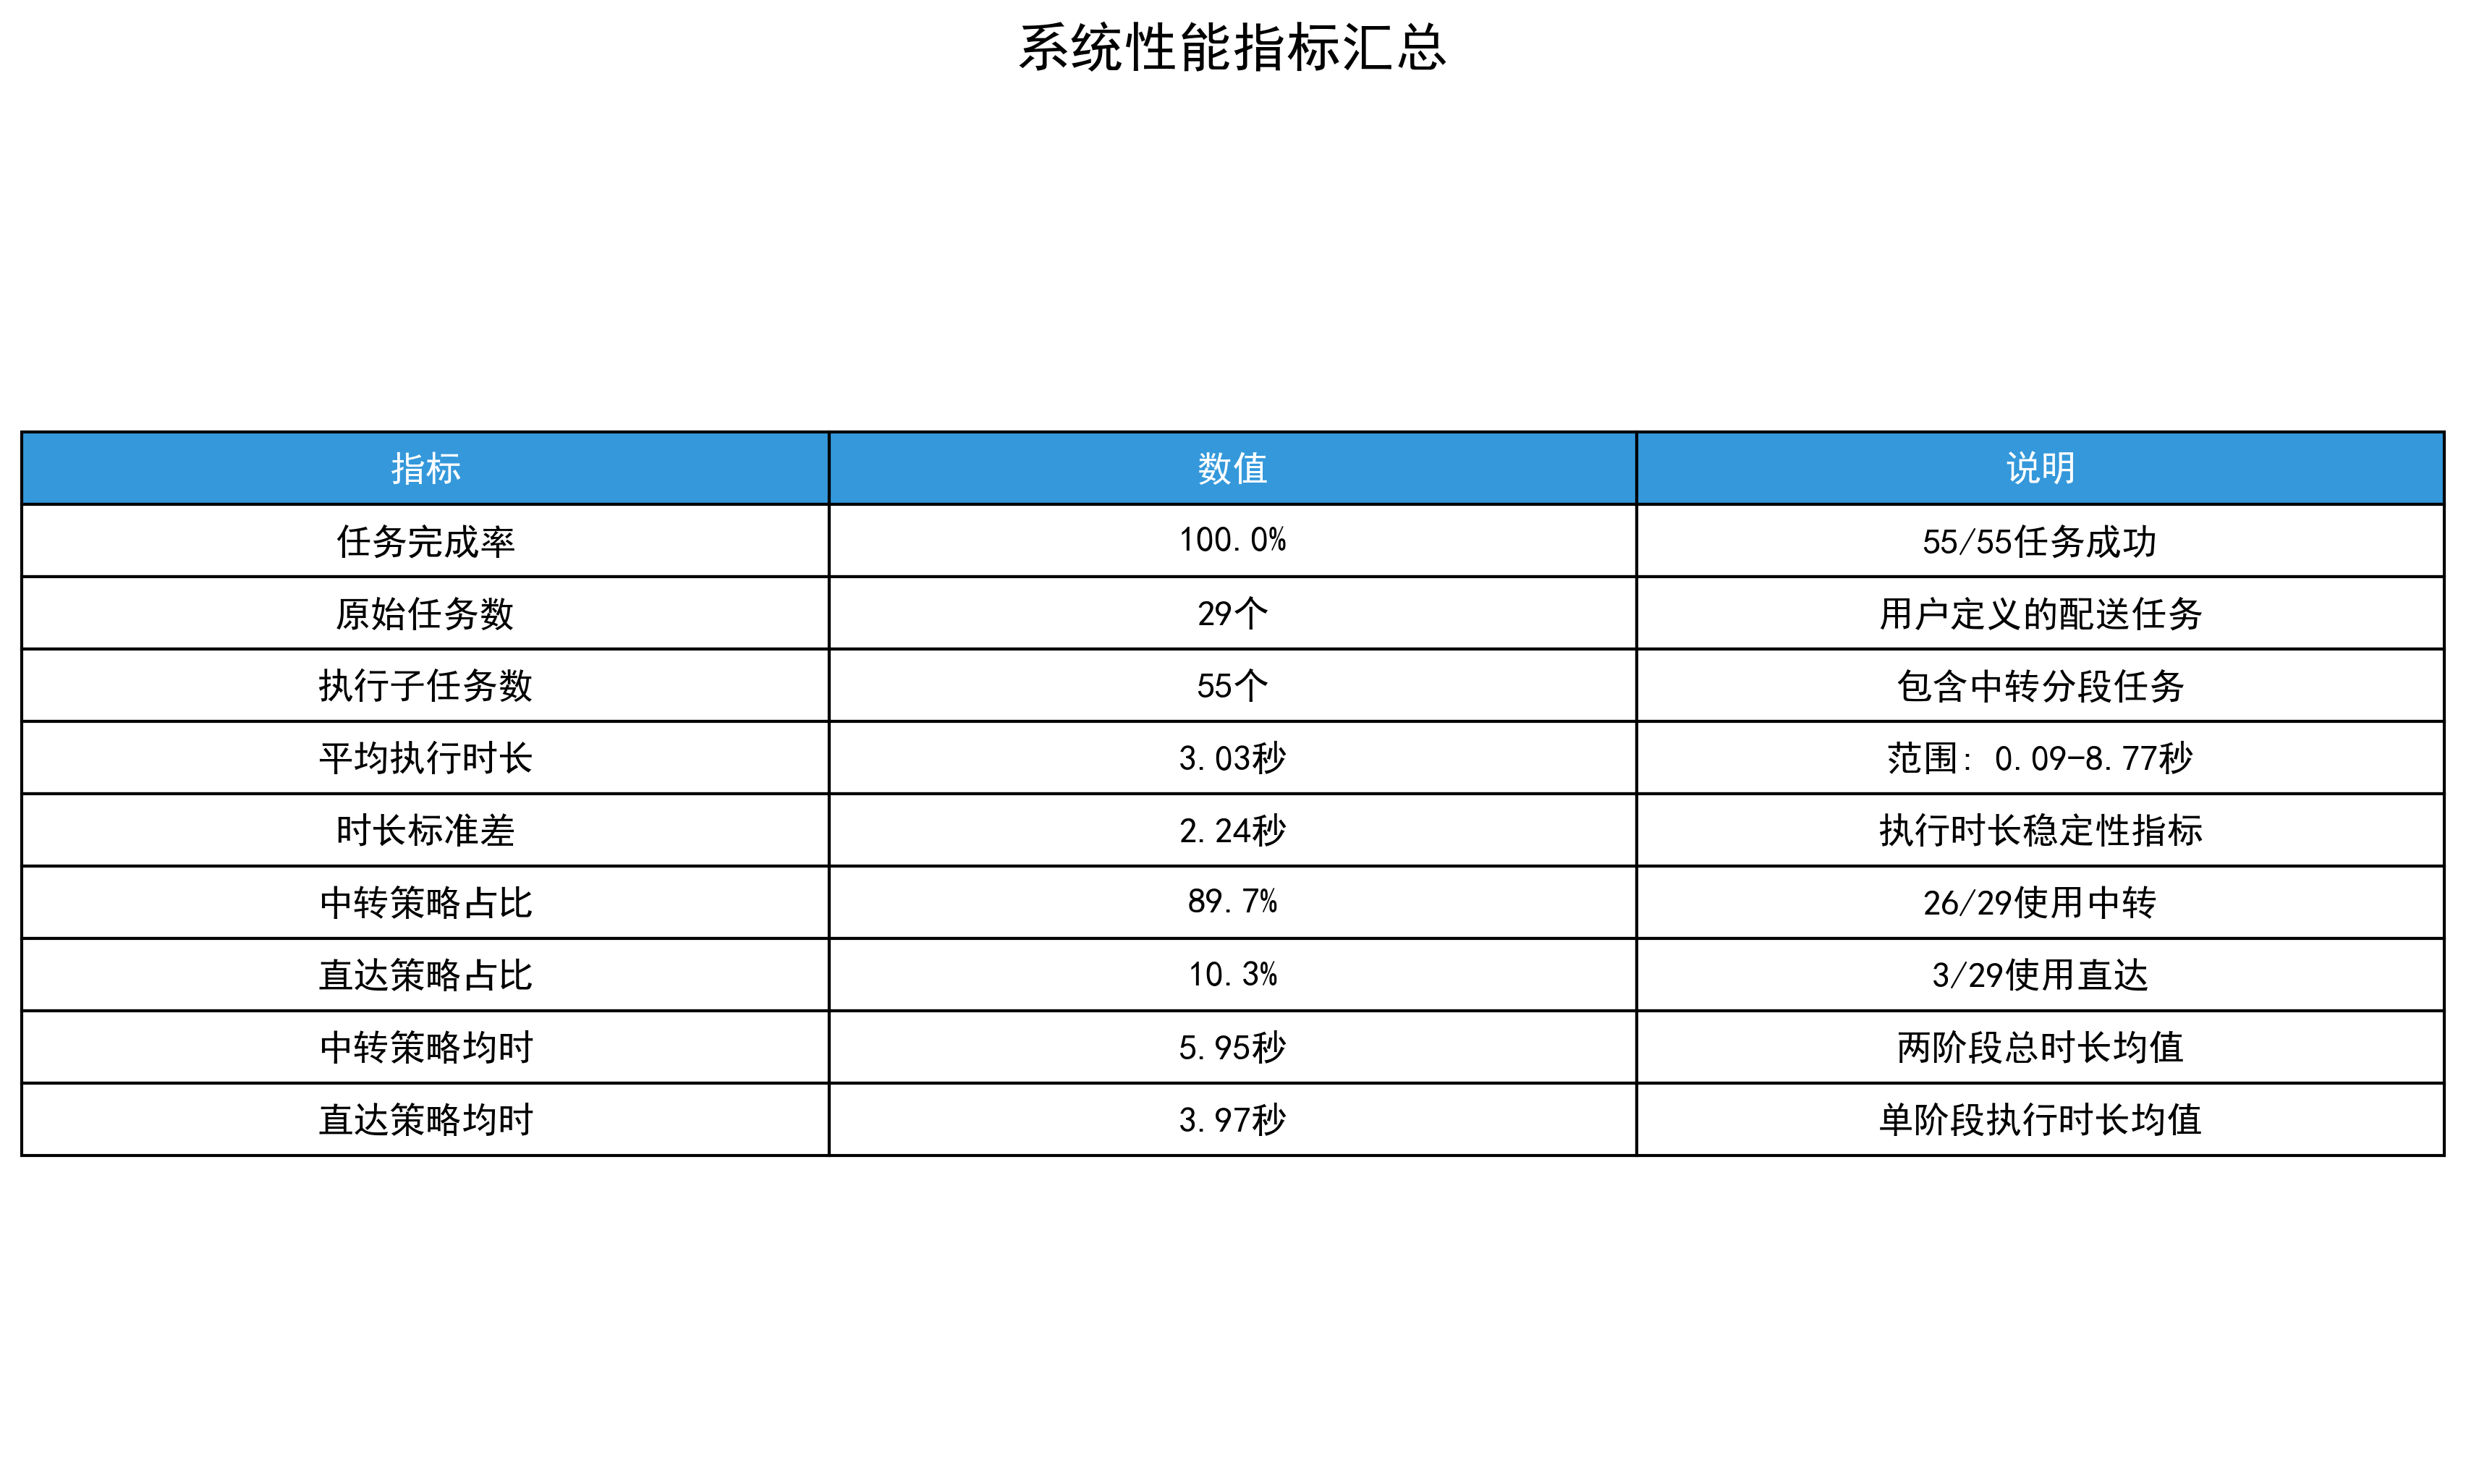
\includegraphics[width=\textwidth]{analysis_results/system_performance_table_20250617_081500.png}
        \caption{系统性能指标汇总表}
    \end{figure}
\end{frame}

\begin{frame}{智能体性能对比分析}
    \begin{figure}
        \centering
        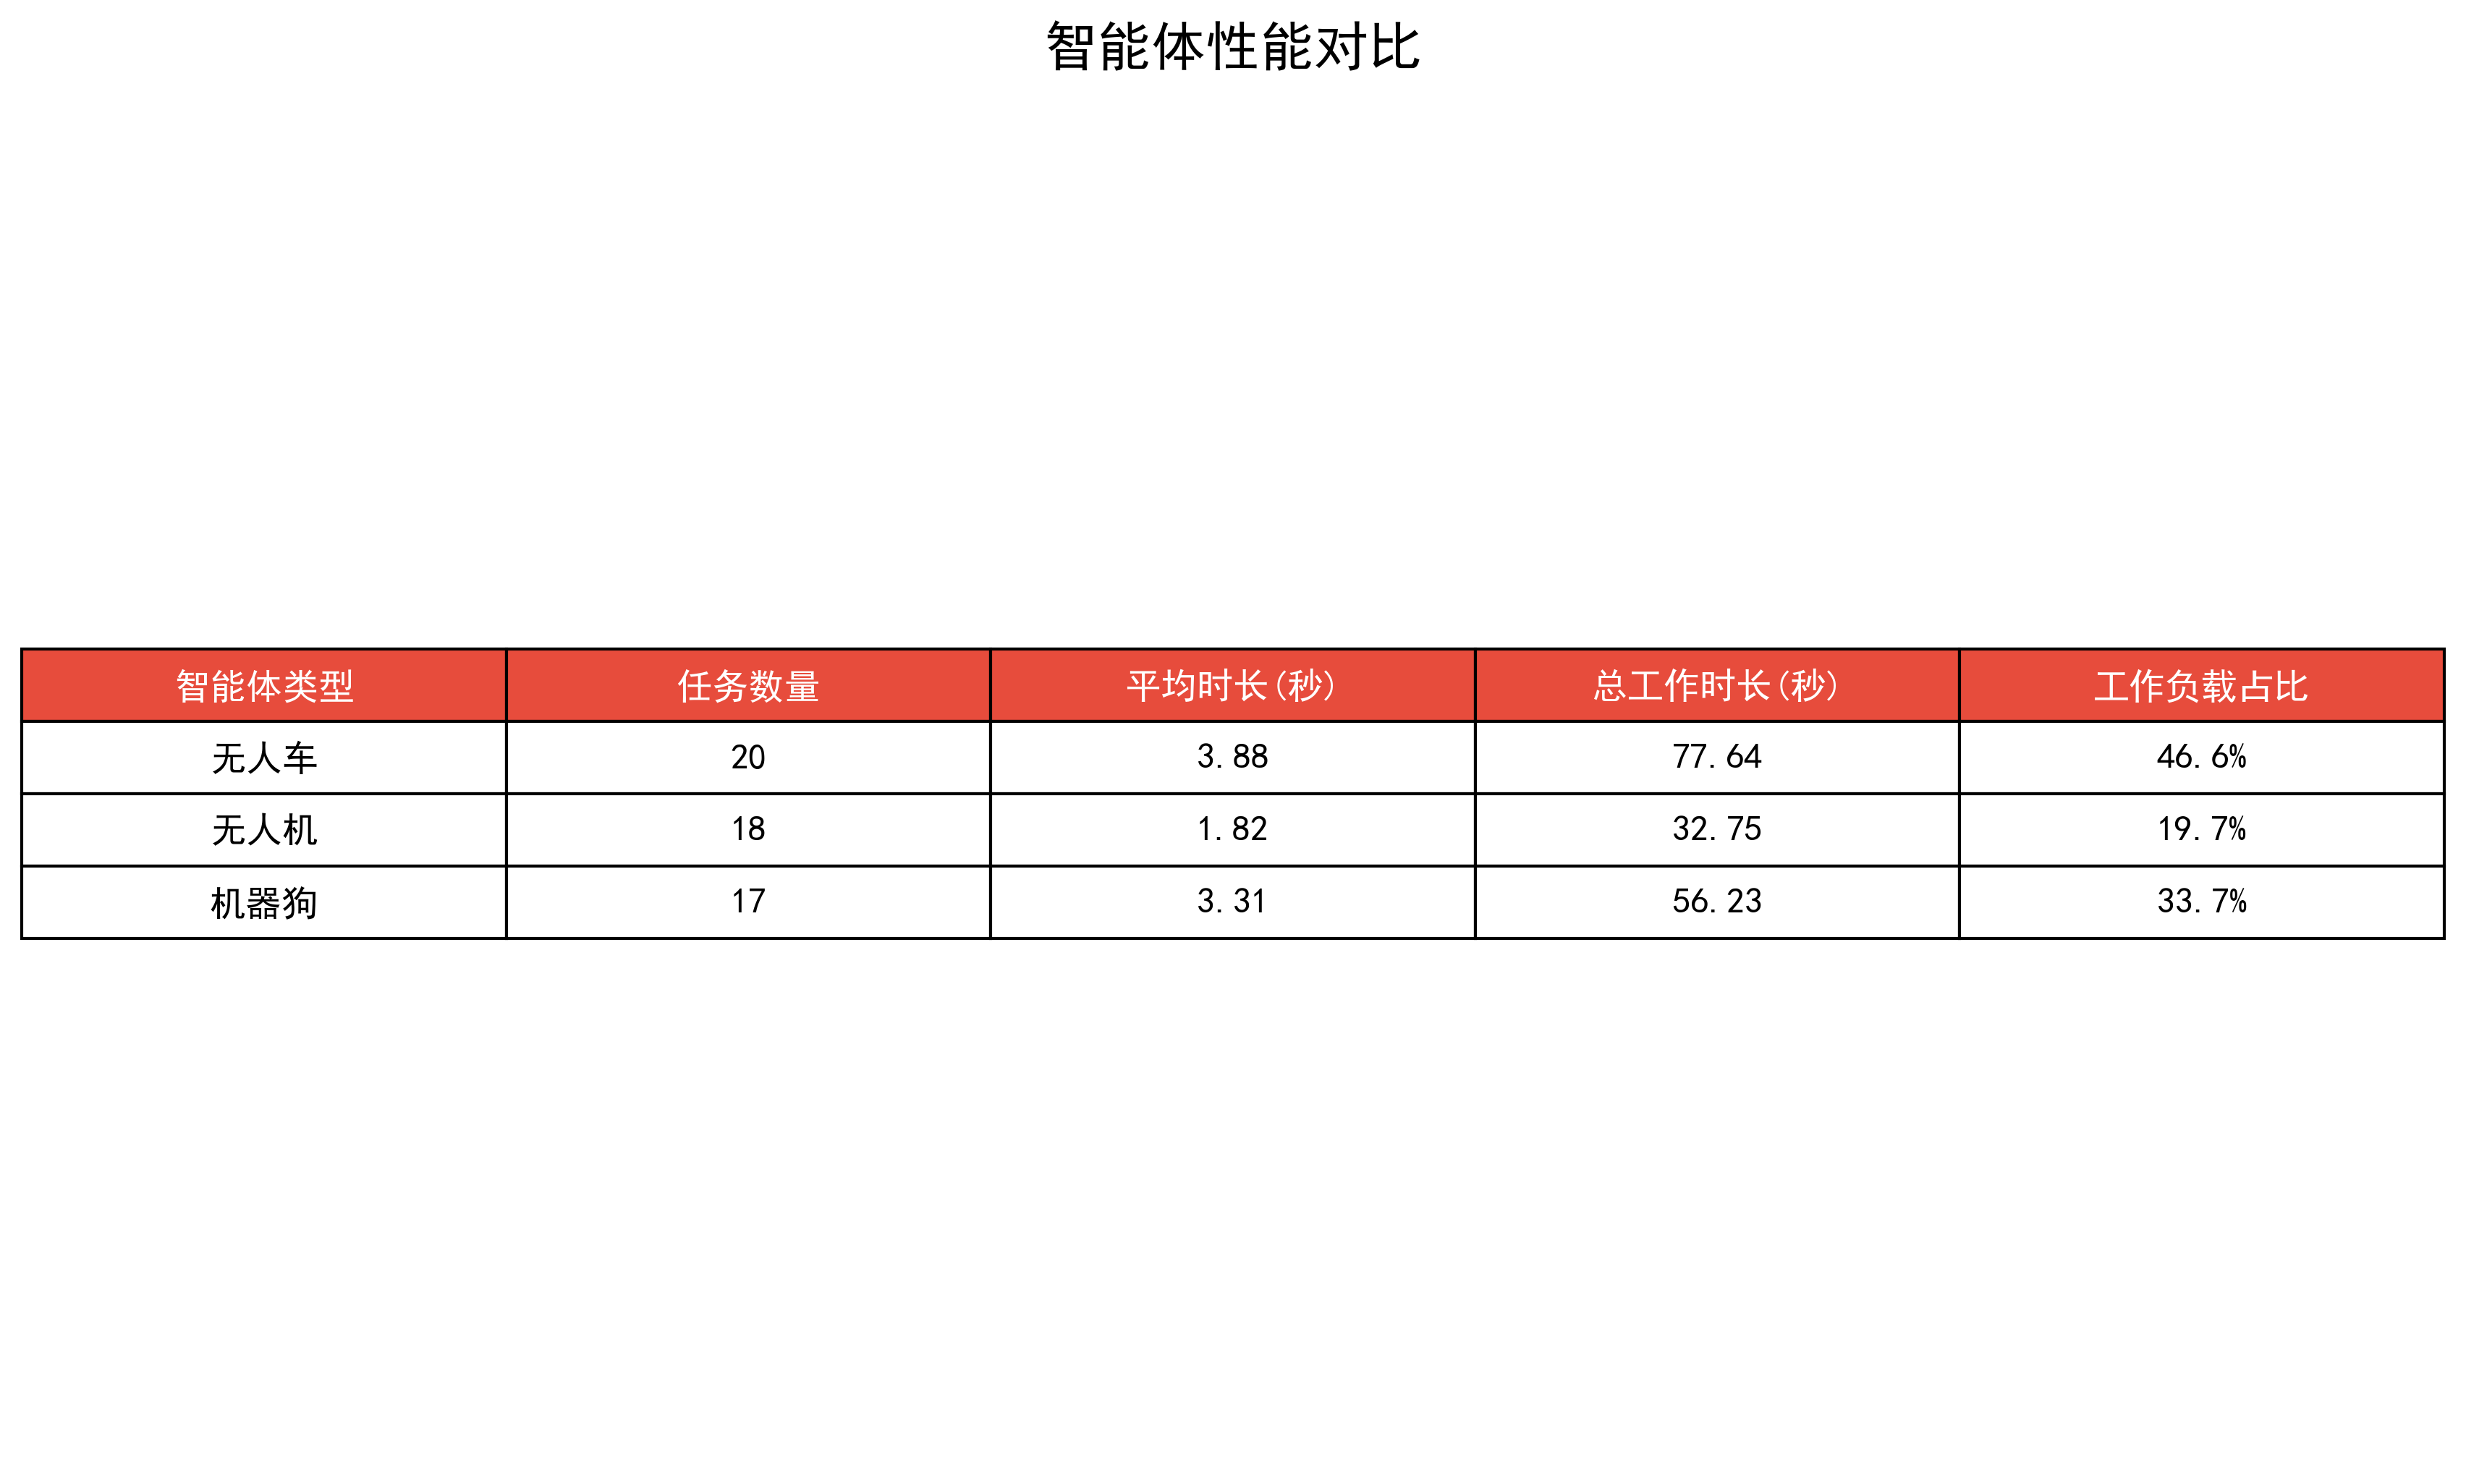
\includegraphics[width=0.9\textwidth]{analysis_results/agent_performance_table_20250617_081500.png}
        \caption{各类型智能体性能对比表}
    \end{figure}
    
    \begin{columns}
        \begin{column}{0.5\textwidth}
            \begin{exampleblock}{效率对比}
                \begin{itemize}
                    \item \textbf{无人机}:平均执行时长最短(1.67秒)
                    \item \textbf{无人车}:平均执行时长最长(3.91秒)
                    \item \textbf{机器狗}:平均执行时长适中(3.22秒)
                \end{itemize}
            \end{exampleblock}
        \end{column}
        \begin{column}{0.5\textwidth}
            \begin{alertblock}{工作负载分析}
                \begin{itemize}
                    \item 负载均衡度:\textbf{96.8\%}
                    \item 总工作时长占比:无人机(28.3\%)、无人车(37.7\%)、机器狗(34.0\%)
                    \item 资源利用优化:系统根据任务特性合理分配载具
                \end{itemize}
            \end{alertblock}
        \end{column}
    \end{columns}
\end{frame}

\subsection{系统可视化展示}
\begin{frame}{系统运行可视化截图(1)}
    \begin{figure}
        \centering
        \begin{minipage}[t]{0.3\textwidth}
            \centering
            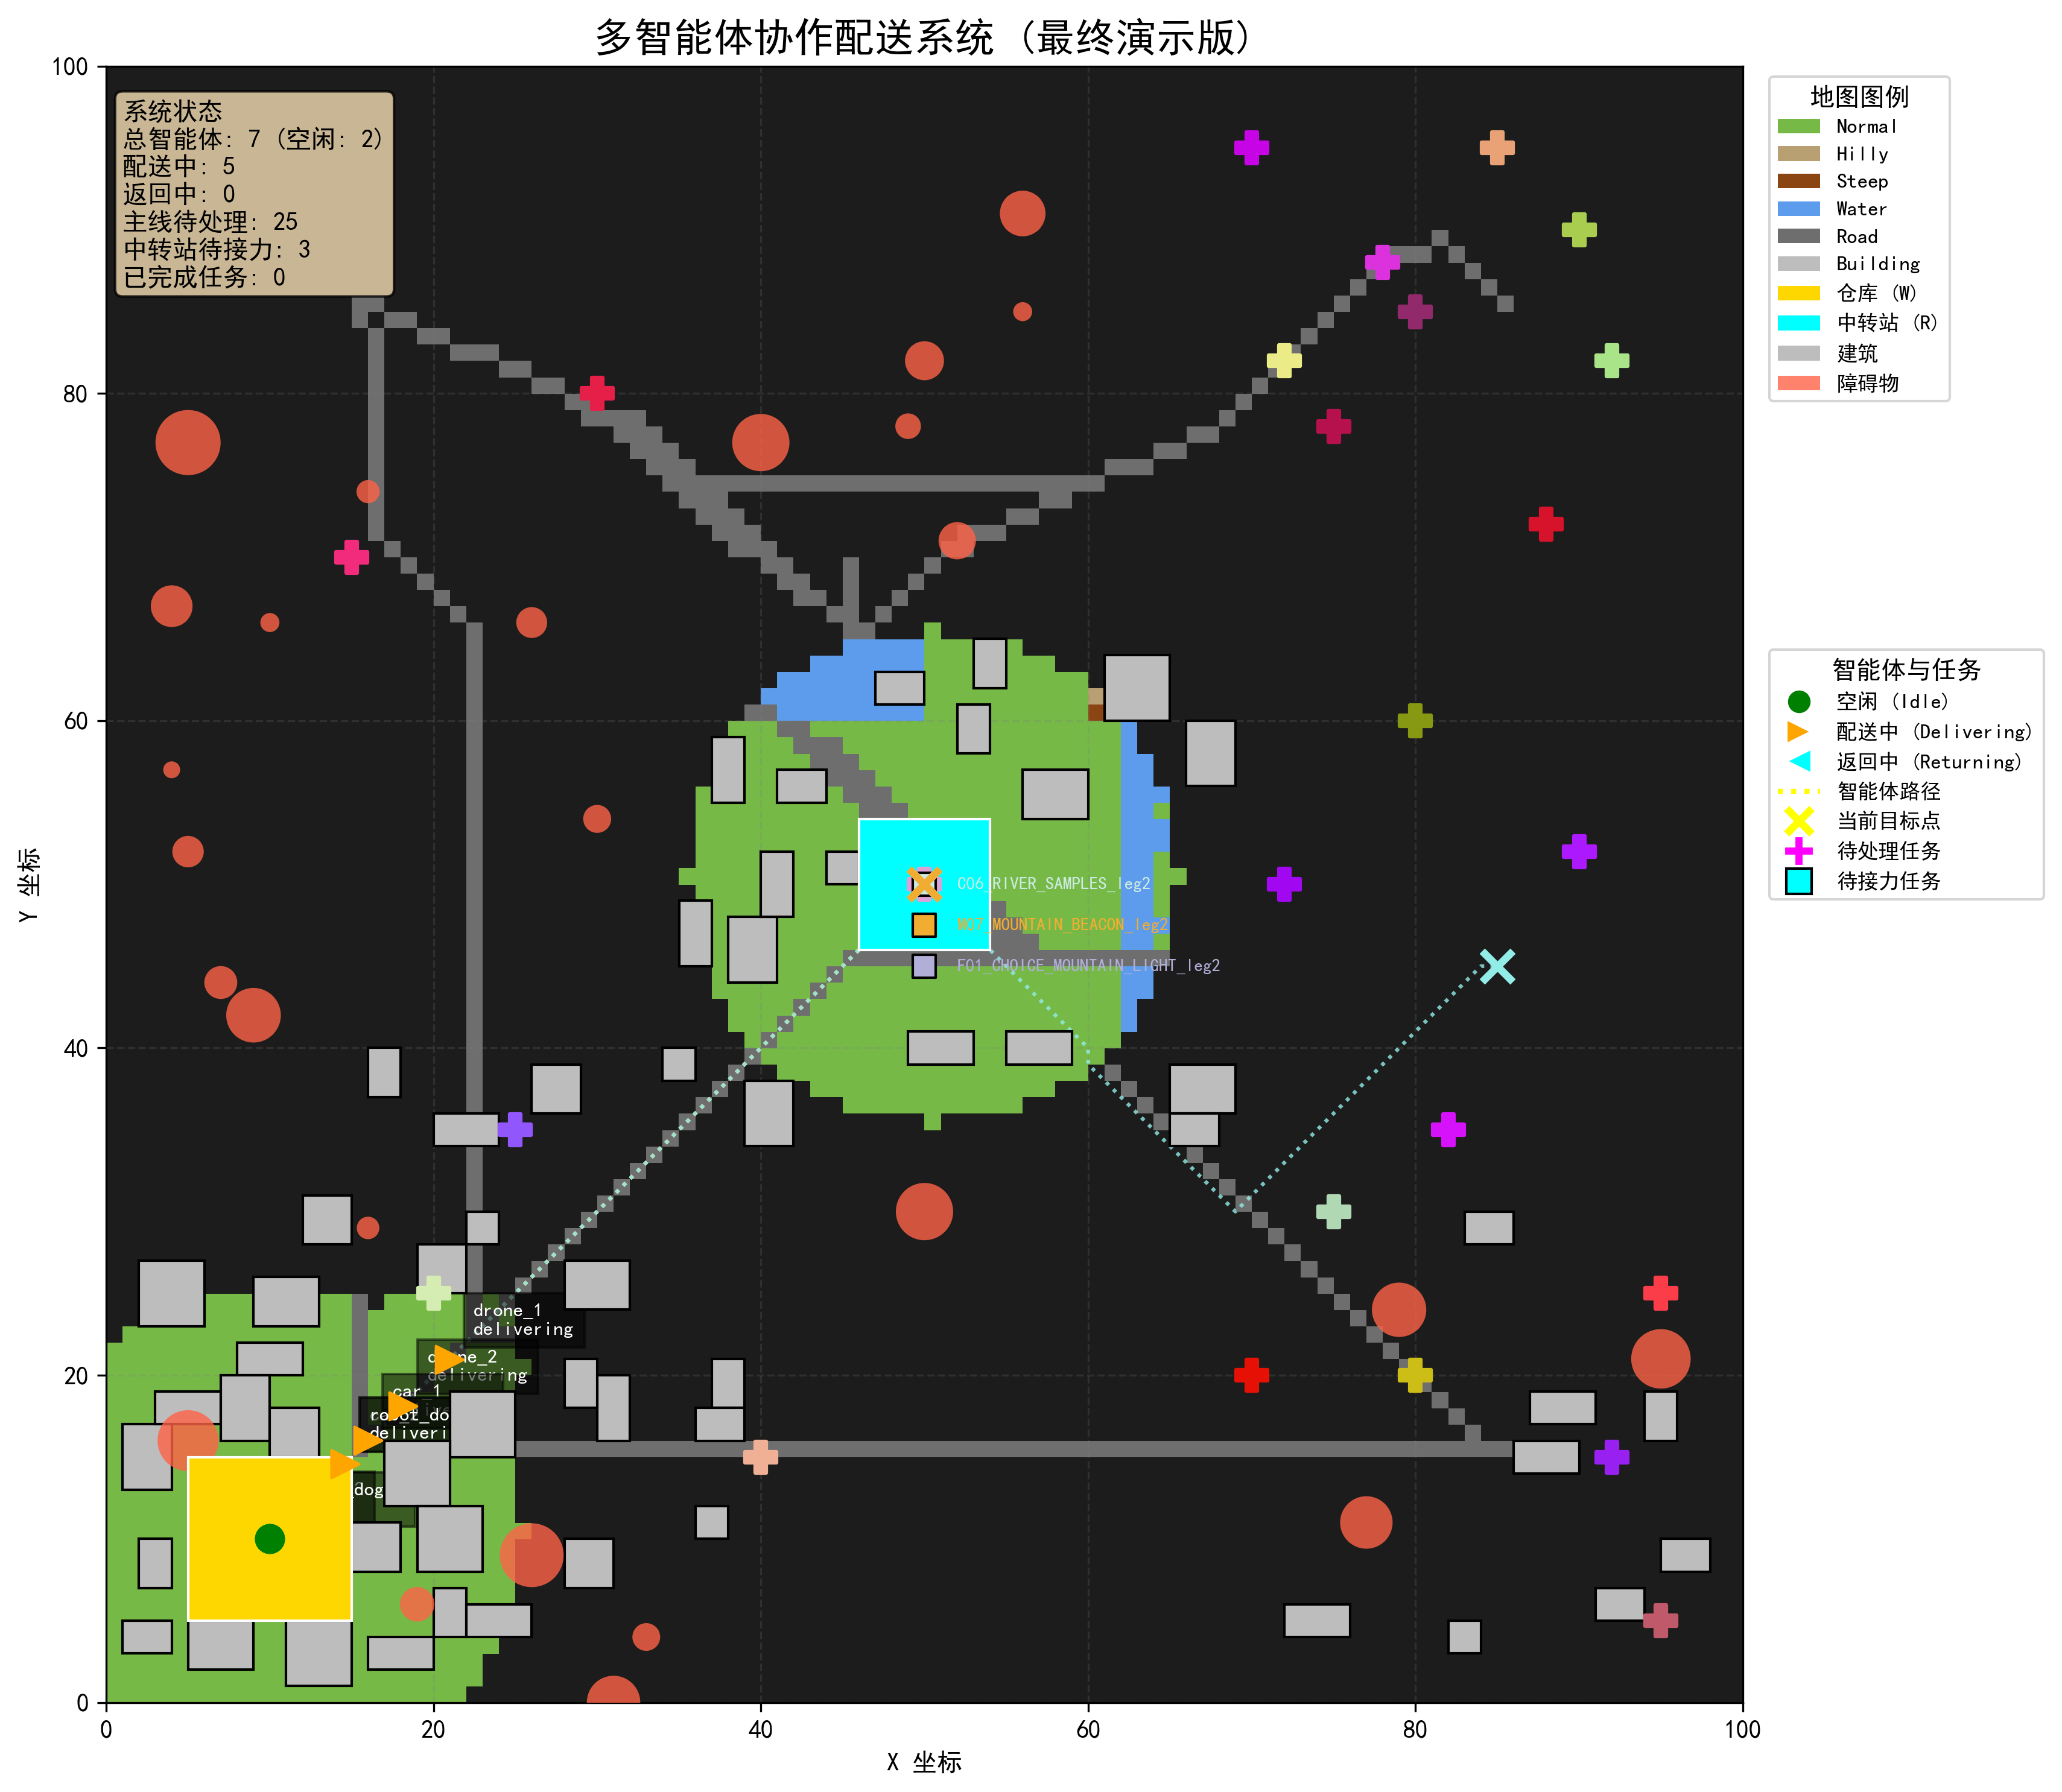
\includegraphics[width=\textwidth]{visualization_snapshots/1.png}
            \caption{初始状态}
        \end{minipage}
        \hfill
        \begin{minipage}[t]{0.3\textwidth}
            \centering
            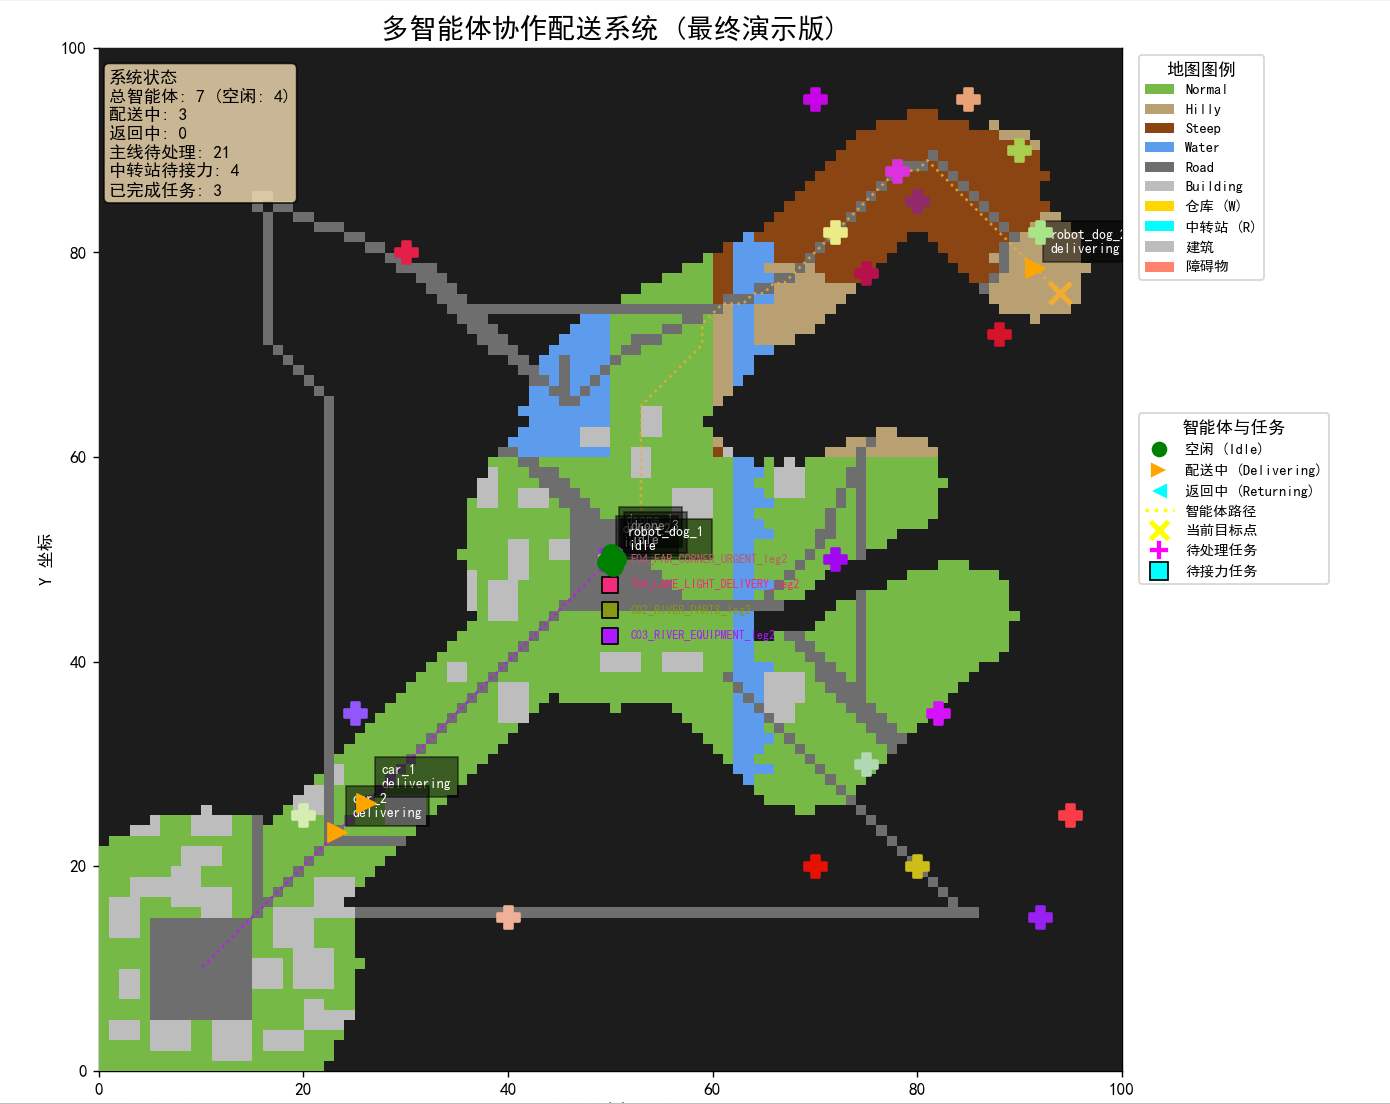
\includegraphics[width=\textwidth]{visualization_snapshots/2.png}
            \caption{任务分配}
        \end{minipage}
        \hfill
        \begin{minipage}[t]{0.3\textwidth}
            \centering
            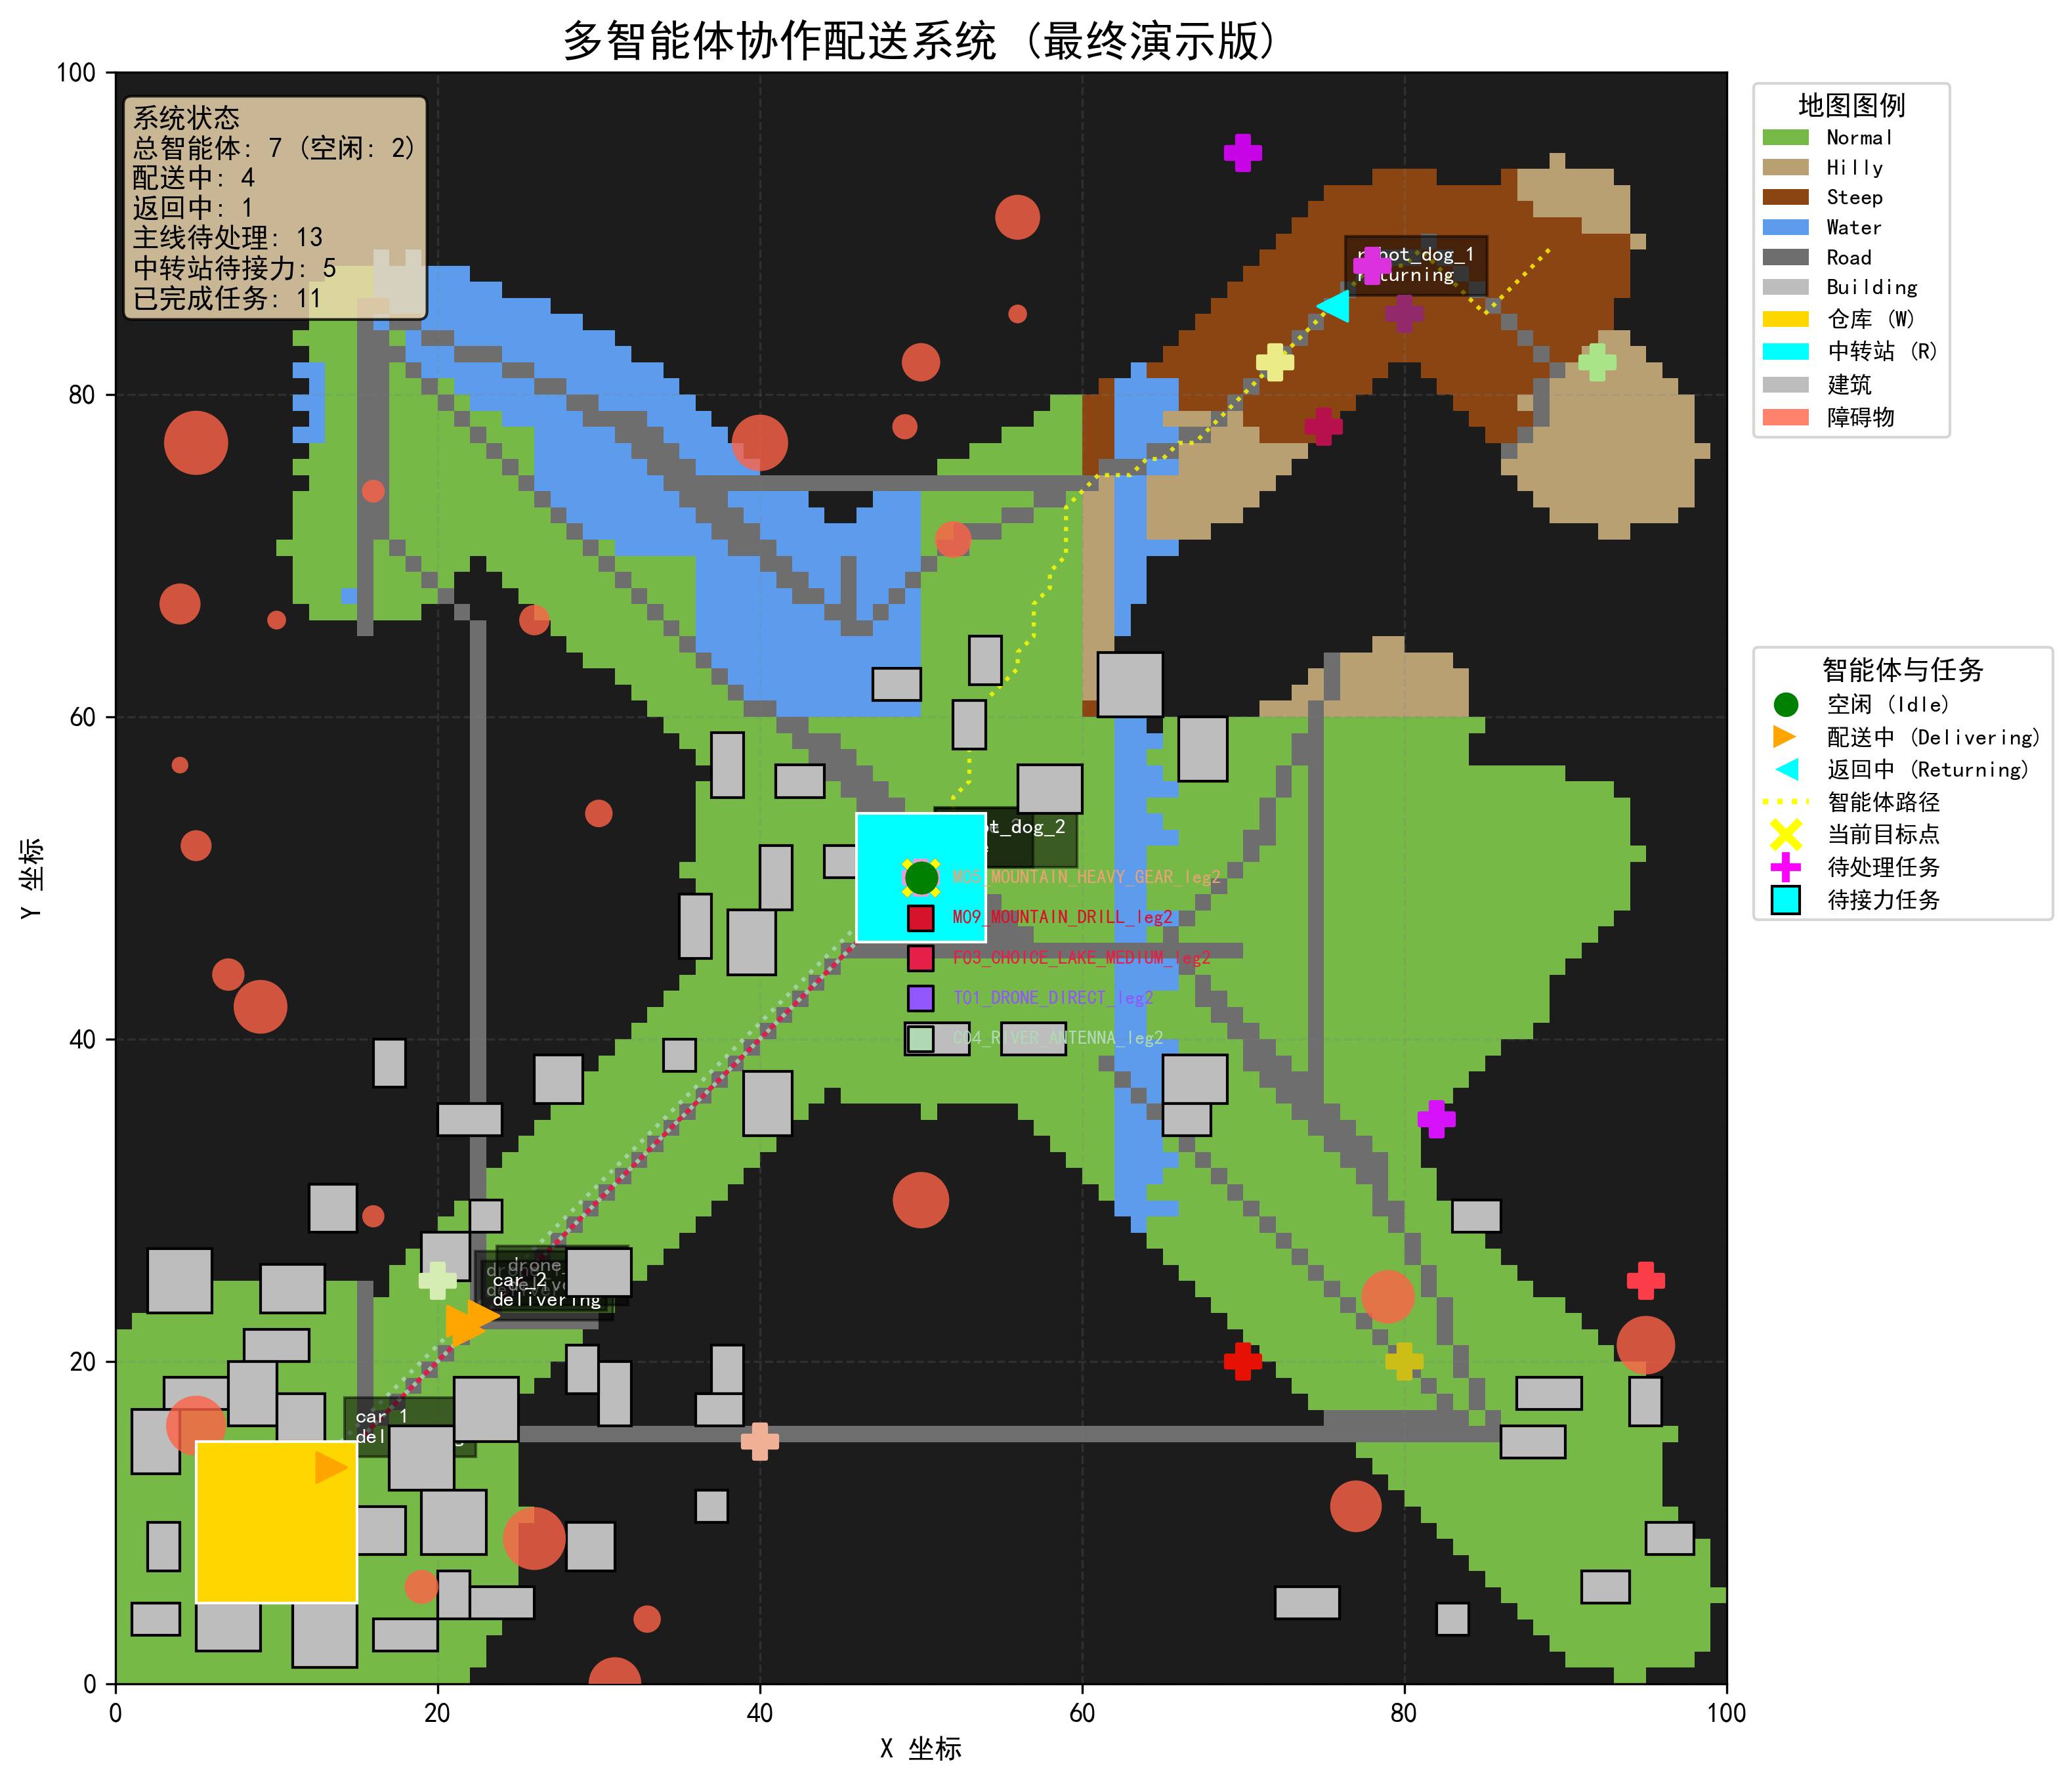
\includegraphics[width=\textwidth]{visualization_snapshots/3.png}
            \caption{协作配送}
        \end{minipage}
        
        \caption{多智能体协作配送系统运行过程可视化(第一阶段)}
    \end{figure}
\end{frame}

\begin{frame}{系统运行可视化截图(2)}
    \begin{figure}
        \centering
        \begin{minipage}[t]{0.4\textwidth}
            \centering
            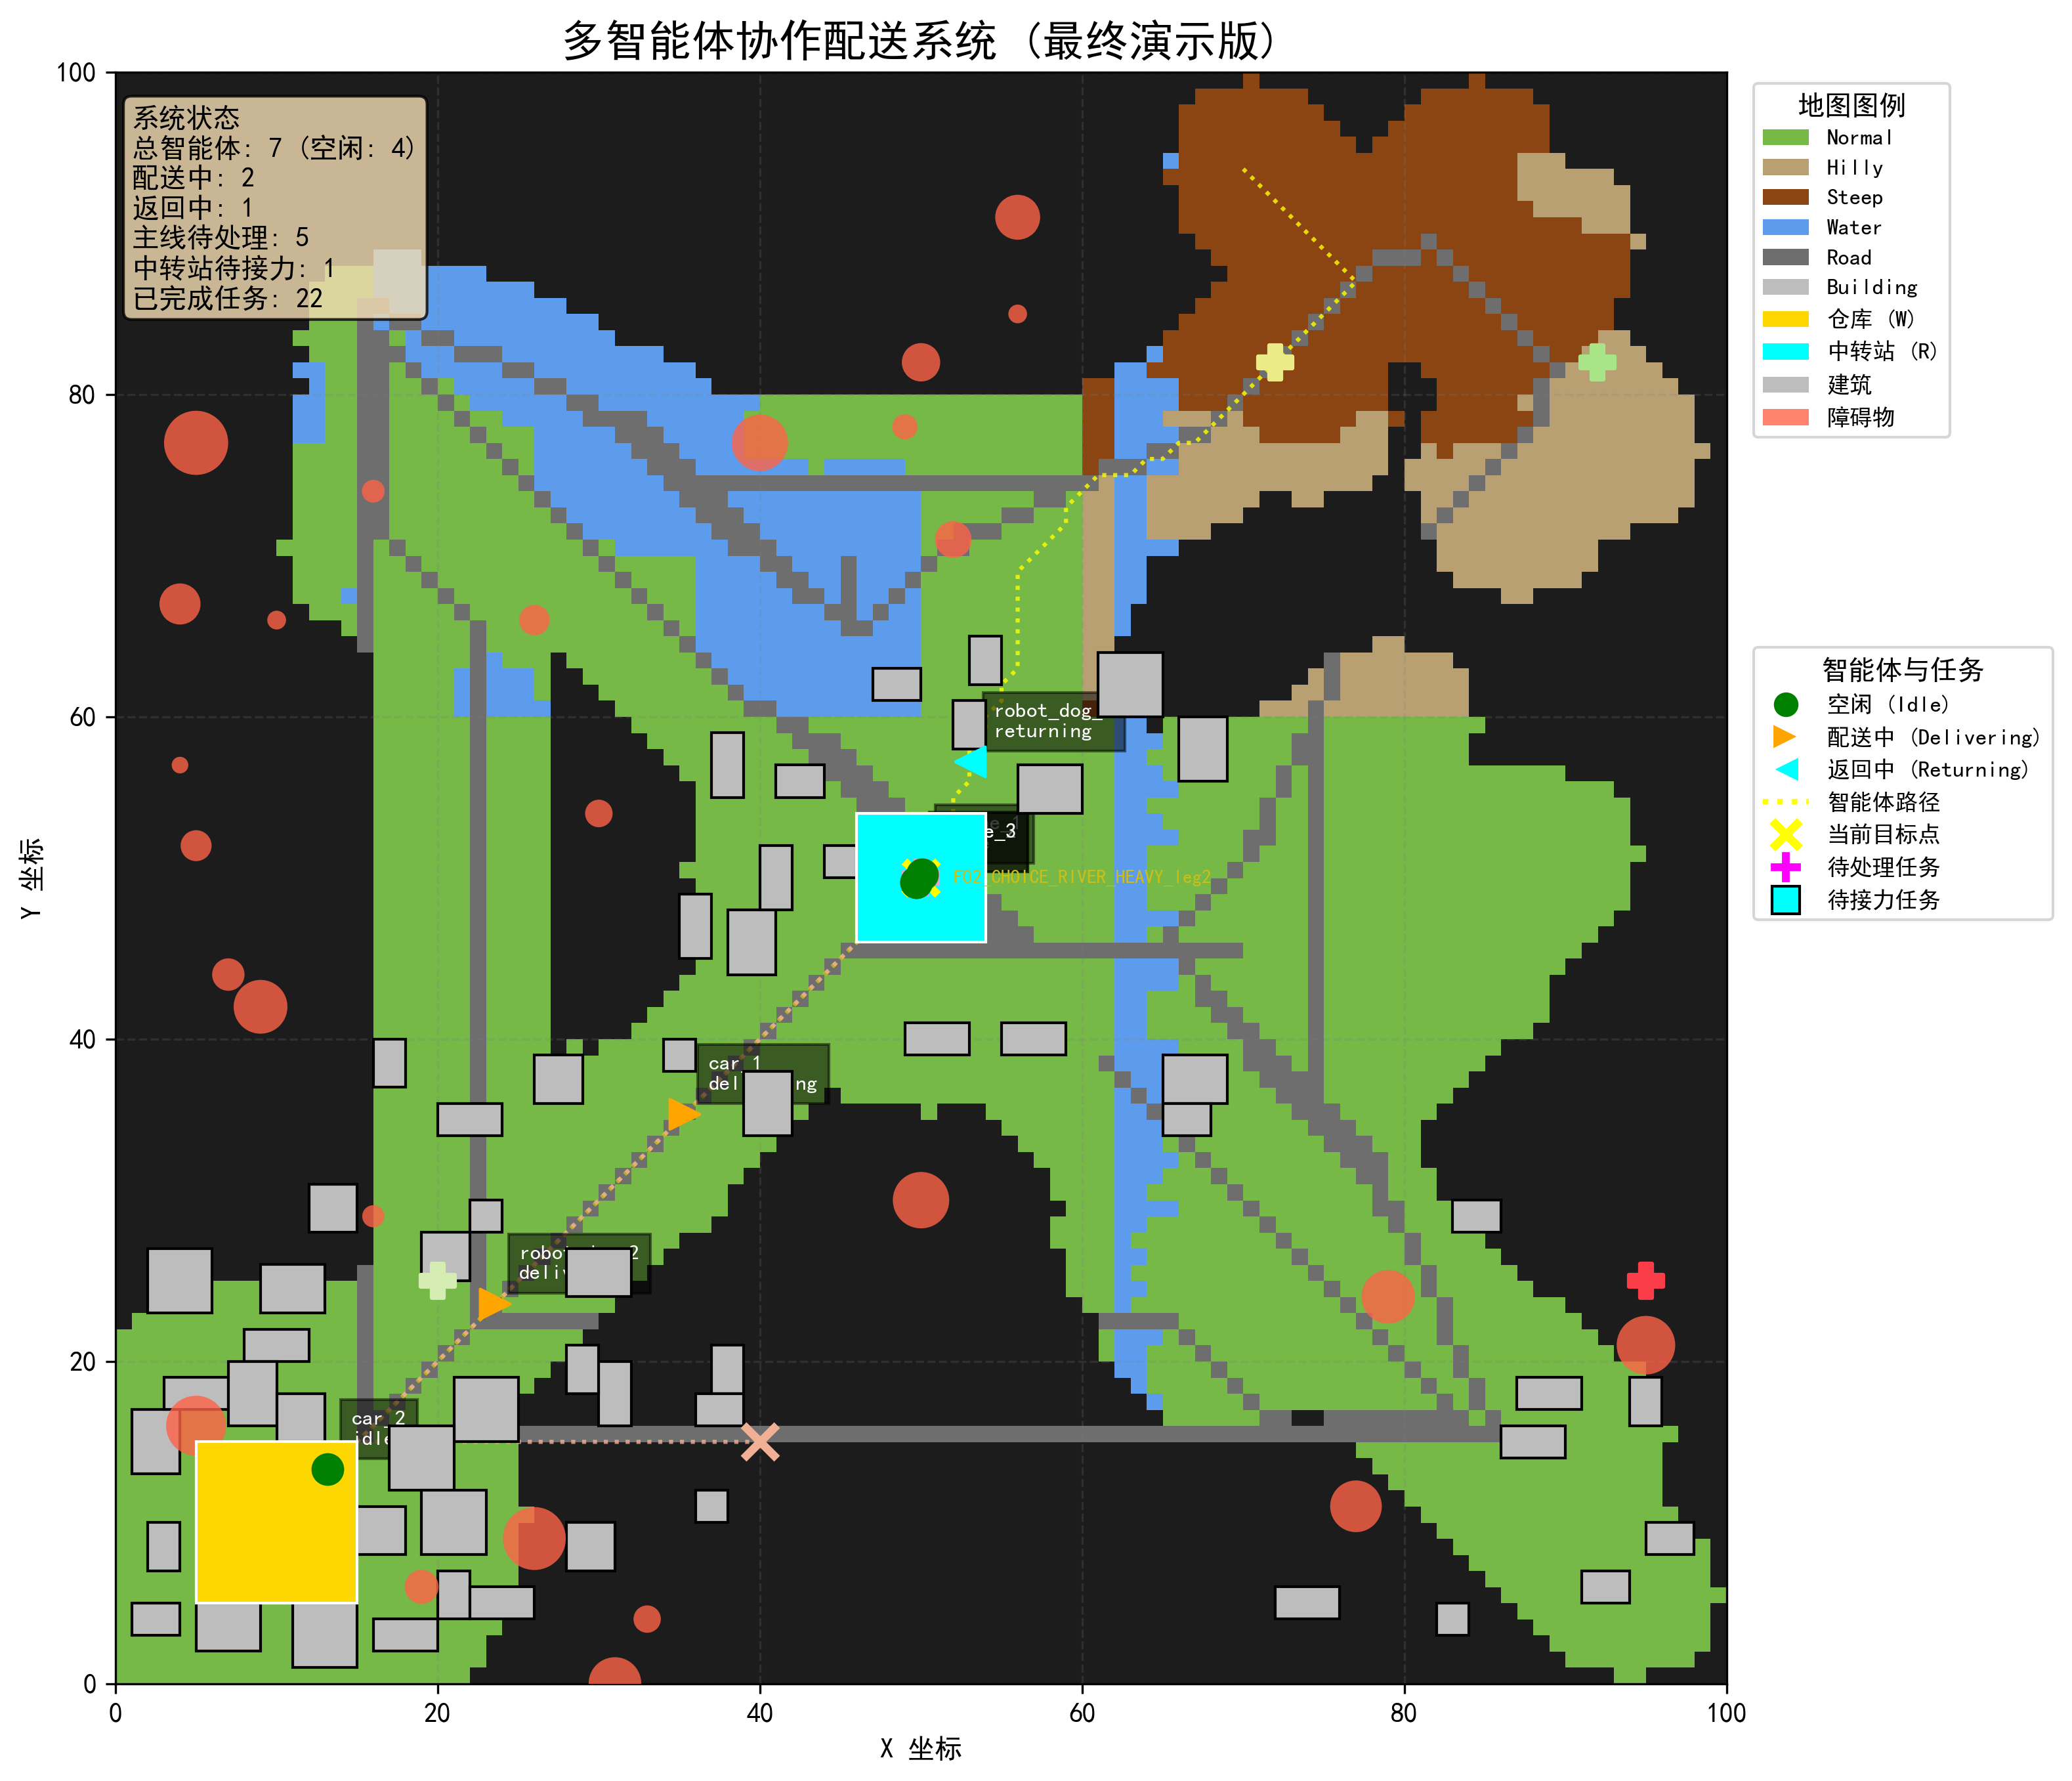
\includegraphics[width=\textwidth]{visualization_snapshots/4.png}
            \caption{中转执行}
        \end{minipage}
        \hfill
        \begin{minipage}[t]{0.4\textwidth}
            \centering
            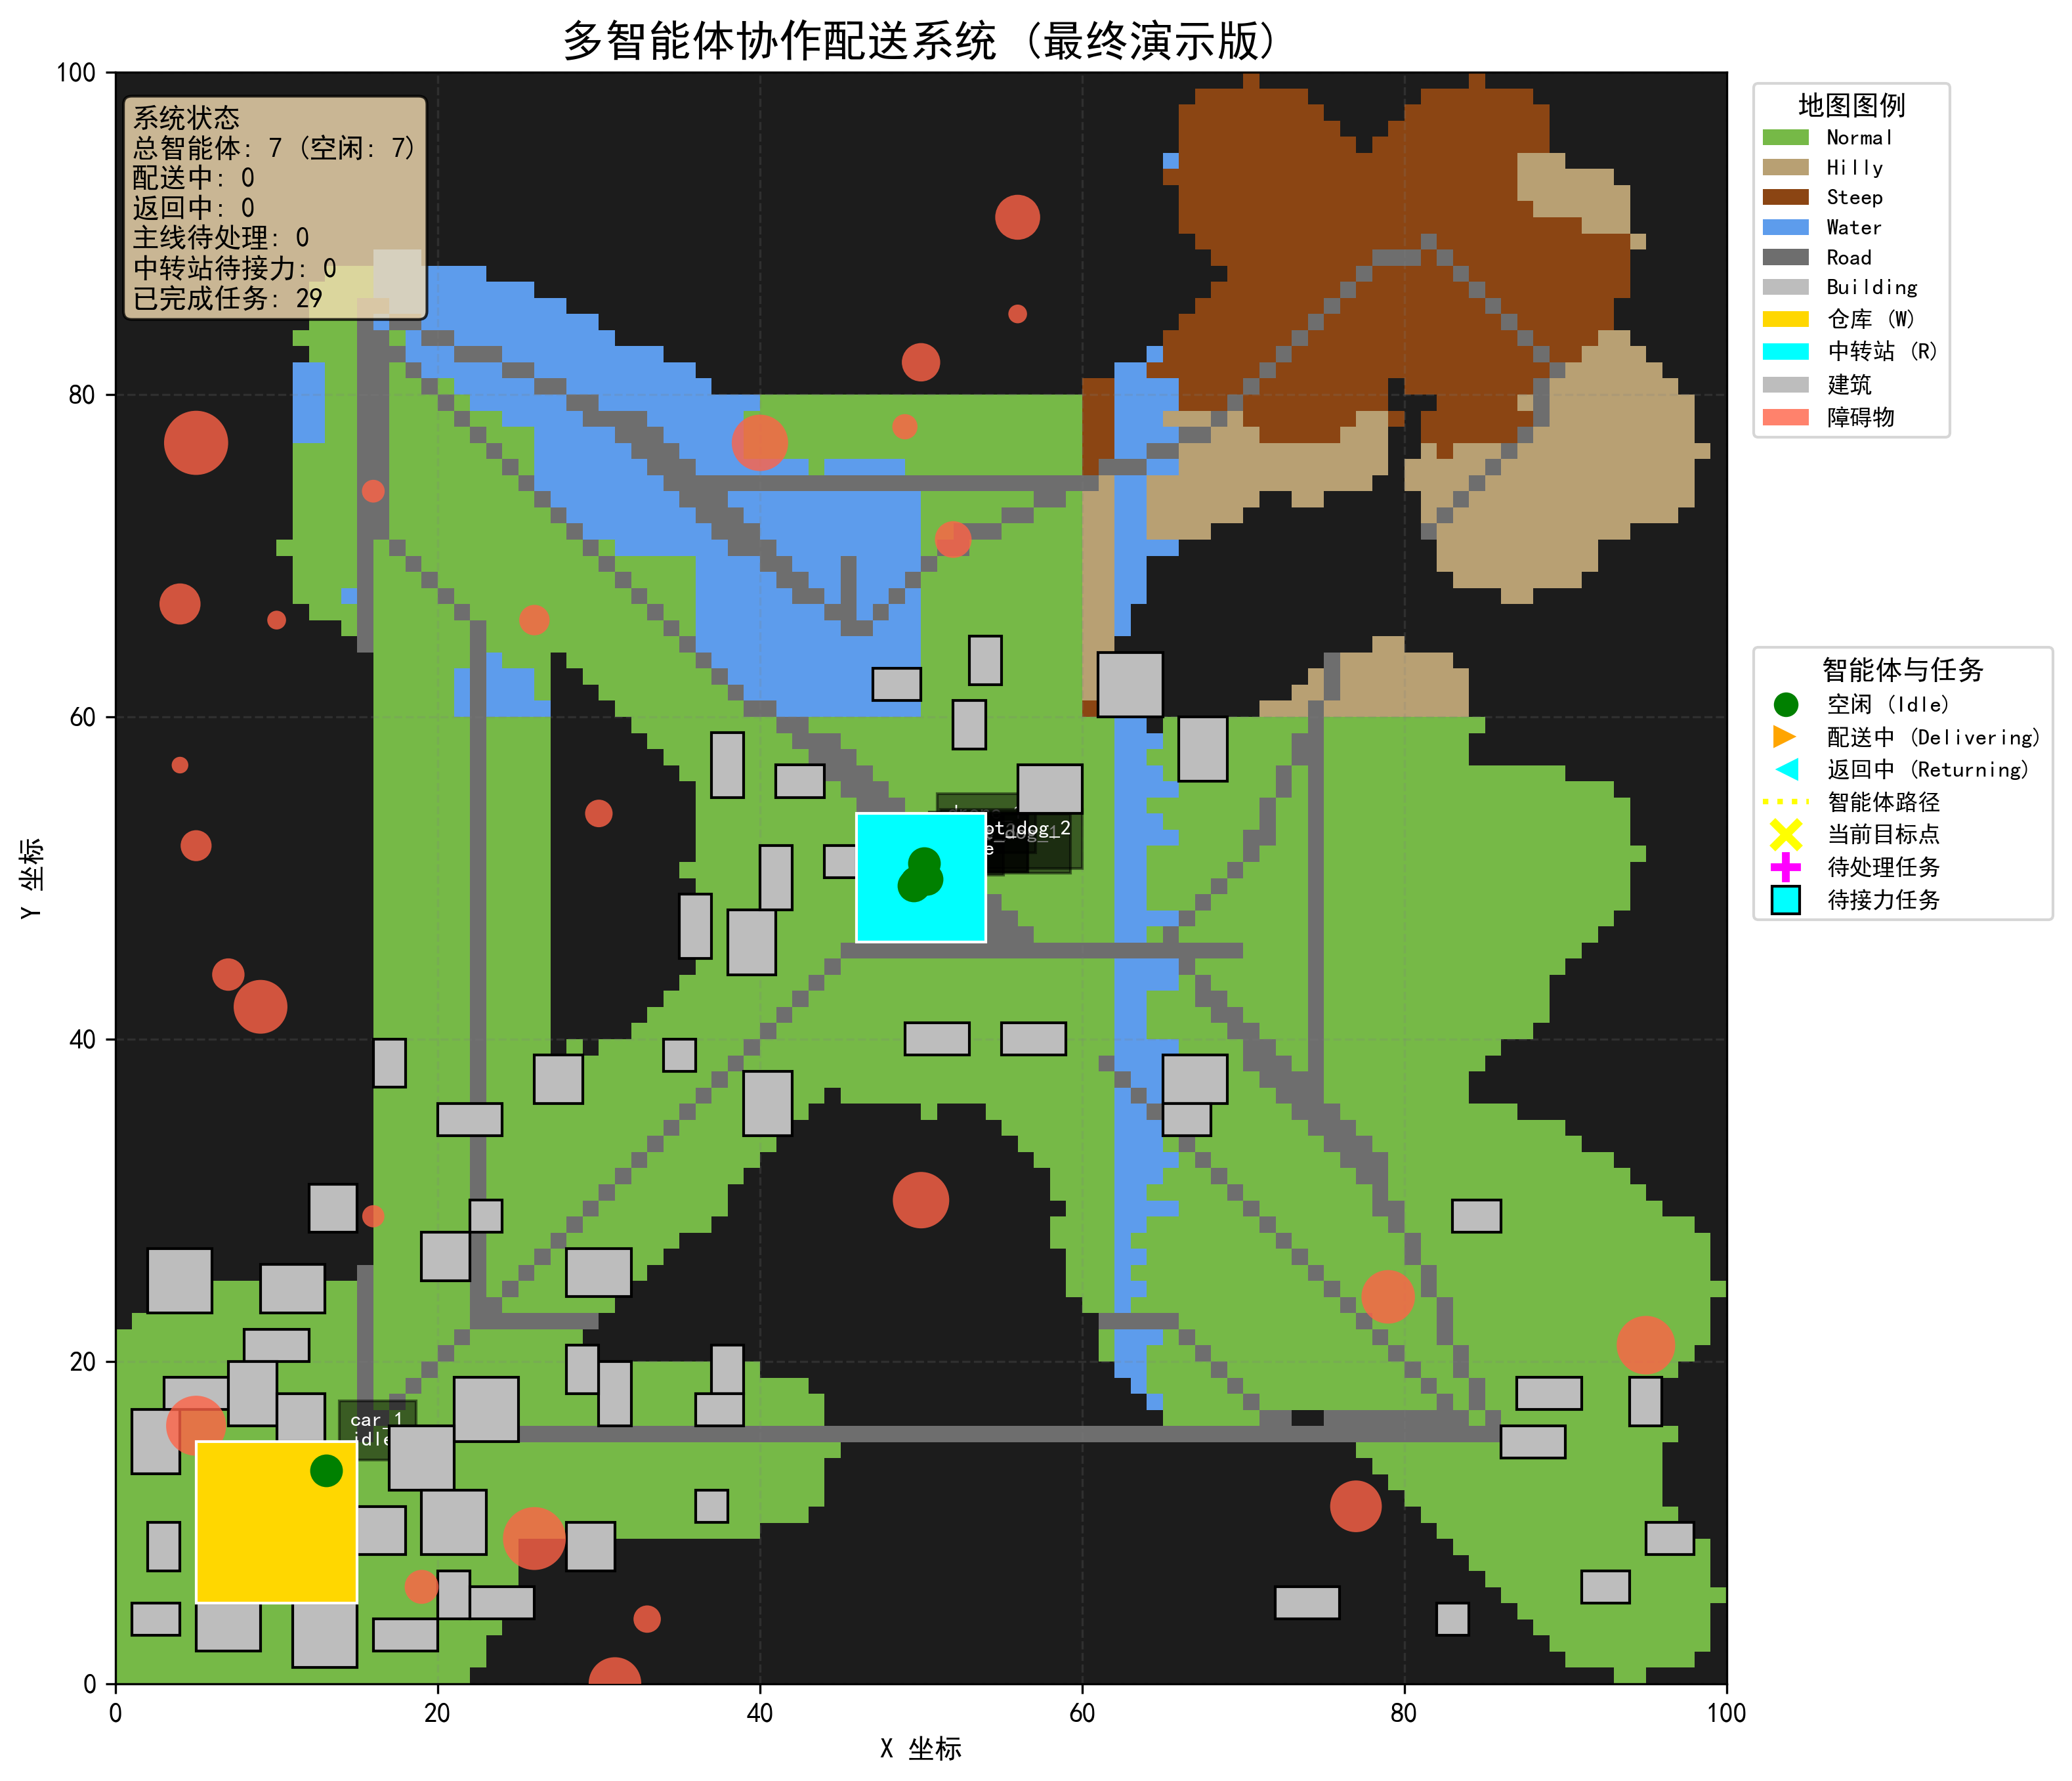
\includegraphics[width=\textwidth]{visualization_snapshots/5.png}
            \caption{任务完成}
        \end{minipage}
        
        \caption{多智能体协作配送系统运行过程可视化(第二阶段)}
    \end{figure}
\end{frame}

\section{总结与展望}

\begin{frame}{项目总结与贡献}
    \begin{block}{主要技术贡献}
        \begin{itemize}
            \item \textbf{异构智能体协作框架}:设计了三种载具的协同工作机制
            \item \textbf{双策略智能决策算法}:实现了直达与中转的最优策略选择
            \item \textbf{战争迷雾探索系统}:建立了有限视野下的协作式地图构建
            \item \textbf{实时仿真平台}:开发了高性能可视化与监控系统
        \end{itemize}
    \end{block}
    
    \begin{columns}
        \begin{column}{0.5\textwidth}
            \begin{exampleblock}{应用前景}
                \begin{itemize}
                    \item 智慧城市物流配送
                    \item 应急救援物资投送
                    \item 偏远地区服务覆盖
                    \item 多机器人系统研究
                \end{itemize}
            \end{exampleblock}
        \end{column}
        \begin{column}{0.5\textwidth}
            \begin{alertblock}{未来工作}
                \begin{itemize}
                    \item 强化学习优化决策
                    \item 动态环境事件处理
                    \item 能耗模型与充电规划
                    \item 大规模系统扩展验证
                \end{itemize}
            \end{alertblock}
        \end{column}
    \end{columns}
    
    \begin{center}
        \Large \textbf{谢谢大家!欢迎交流讨论}
    \end{center}
\end{frame}

\begin{frame}{未来研究方向的数学建模}
    \begin{columns}
        \begin{column}{0.5\textwidth}
            \begin{exampleblock}{强化学习框架}
                Q-学习更新公式:
                \begin{align}
                Q(s,a) &\leftarrow (1-\alpha)Q(s,a) + \alpha[r + \gamma \max_{a'}Q(s',a')] \\
                \end{align}
                
                策略改进:
                \begin{align}
                \pi(s) &= \arg\max_a Q(s,a) \\
                P(a|s) &= \frac{e^{Q(s,a)/\tau}}{\sum_{a'} e^{Q(s,a')/\tau}} \quad \text{(软性选择)}
                \end{align}
            \end{exampleblock}
        \end{column}
        \begin{column}{0.5\textwidth}
            \begin{alertblock}{能耗模型与充电规划}
                能耗函数:
                \begin{align}
                E(d,w,v,\alpha) &= E_{base} + k_1 \cdot d + k_2 \cdot w + k_3 \cdot v^2 + k_4 \cdot \alpha\\
                \end{align}
                其中:$d$为距离,$w$为负载,$v$为速度,$\alpha$为地形系数
                
                充电决策阈值:
                \begin{align}
                \text{NeedCharge} &= 
                \begin{cases}
                \text{True}, & \text{if } E_{remain} < E_{required} + E_{safety} \\
                \text{False}, & \text{otherwise}
                \end{cases}
                \end{align}
            \end{alertblock}
        \end{column}
    \end{columns}
    
    \begin{block}{多目标优化模型}
        目标函数:
        \begin{align}
        \min F(x) &= (f_1(x), f_2(x), ..., f_k(x))^T \\
        f_1(x) &= \text{总配送时间} \\
        f_2(x) &= \text{总能耗} \\
        f_3(x) &= \text{资源利用不平衡度} \\
        \end{align}
        
        Pareto最优解集:$P^* = \{x \in \Omega | \nexists x' \in \Omega, F(x') \prec F(x) \}$
    \end{block}
\end{frame}

\end{document}





